\chapter{Calcul des impôts et crédits}
\section{Introduction et objectifs}
\subsection{Introduction}
Jusqu'à maintenant, vous avez appris comment déclarer les types de revenus que l'on rencontre le plus souvent et comment réclamer certaines déductions et crédits. Ce chapitre explique le calcul de l'impôt. Nous traiterons d'abord le calcul de l'impôt fédéral et, ensuite, le calcul de l'impôt du Québec.


\subsection{Objectifs}
\begin{itemize}[label=\twemoji{check mark button}]
	\item Calculer l'impôt à payer, au fédéral et au Québec;
	\item Calculer le crédit d'impôt pour contributions politiques, au fédéral et au Québec;
	\item Calculer le crédit d'impôt relatif à un fonds de travailleurs, au fédéral et au Québec;
	\item Expliquer le crédit d'impôt pour fournitures scolaires d'éducateur admissible et comment le réclamer;
	\item Établir le montant de la cotisation qu'un contribuable doit payer au Régime d'assurance médicaments du Québec;
	\item Compléter les déclarations de revenus, au fédéral et au Québec.
\end{itemize}


\subsection{Sujets du chapitre}
\begin{itemize}
	\item Fonds de travailleurs
	\item Versement anticipés
	\item Crédit transféré d'un conjoint à l'autre
	\item RAMQ
	\item Remboursement ou solde à payer
\end{itemize}



\section{Calcul de l'impôt fédéral}
\begin{intro}
	Nous continuons maintenant à remplir la partie~C de l'étape 5 de la T1, en appliquant l'impôt fédéral sur le revenu imposable de la partie~A et les crédits non remboursables de la partie~B pour déterminer l'impôt fédéral net.
\end{intro}


\subsection{Impôt fédéral de base (ligne~42900)}
La ligne~42900 est le premier cas où un résultat négatif sera mis à \og 0 \fg{}. Comme indiqué précédemment, si le total des crédits non remboursables dépasse l'impôt à payer, il ne peut être utilisé pour créer un remboursement et les crédits excédentaires seront perdus.


\subsection{Impôt fédéral (ligne~40600)}
La ligne~40600 est un deuxième exemple où un résultat négatif sera mis à \og 0 \fg{}.


\subsection{Impôt fédéral net (ligne~42000)}
Une fois l'impôt fédéral déterminé, nous pouvons appliquer deux autres crédits non remboursables, le crédit d'impôt pour contributions politiques fédérales à la ligne~41000 et le crédit d'impôt relatif à un fonds de travailleurs à la ligne~41400.

\subsubsection{ligne~41700}
Après la demande de crédits pour les contributions politiques et le crédit d'impôt sur les fonds d'investissement, la ligne~41700 est le troisième et dernier cas où un résultat négatif sera mis à  \og 0 \fg{}.

\subsubsection{ligne~41500}
À la ligne~41500, les paiements anticipés reçus par le contribuable au titre de la Prestation pour les travailleurs canadiens seront inscrits. Il s'agit d'un ajout, qui augmente donc l'impôt fédéral net.

\section{Crédit d'impôt pour contribution politique fédérale}
\index{Contribution politique!Fédéral}
Le crédit demandé peut atteindre un maximum de 650~\$, cf. table \ref{table:creditImpotContributionPolitiqueFederale}.
\begin{table}
	\centering
	\arrayrulecolor{ForestGreen}
	\begin{tabular}{ll}
		\textcolor{ForestGreen}{Somme versée} & \textcolor{ForestGreen}{Crédit d'impôt non remboursable} \\ \hline\hline
		400~\$ ou moins                       & 75~\% de la contribution                                 \\ \hline
		Plus de 400~\$ à 750~\$               & 300~\$ plus 50~\% de la contribution excédant de         \\
		& 400~\$ jusqu'à 750~\$                                    \\ \hline
		Plus de 750~\$ à \numprint{1275}~\$   & 475~\$ plus 33,33~\% de la contribution excédant 750~\$  \\ \hline
		\numprint{1275}~\$ et plus            & Déduction maximale de 650~\$                             \\ \hline
	\end{tabular}
	\caption{Crédit d'impôt pour contribution politique fédérale}
	\label{table:creditImpotContributionPolitiqueFederale}
\end{table}

Pour l'année où la contribution est versée, le crédit d'impôt pour les contributions politiques fédérales est applicable jusqu'à concurrence de l'impôt fédéral à payer. 


\subsection{Traitement fiscal}
Le contribuable peut calculer le crédit manuellement ou utiliser la feuille de travail pour la déclaration \og ligne~41000 \fg{}. Par la suite, il entre le montant total des contributions versées à la ligne~40900 de la T1 et le crédit d'impôt pour les contributions politiques fédérales à la ligne~41000 de la T1. Il doit joindre les pièces justificatives à sa déclaration fédérale sur papier.



\section{Crédit d'impôt relatif à un fonds de travailleurs - Fédéral}
\begin{intro}
	Le crédit d'impôt relatif aux fonds de travailleurs peut être demandé par les contribuables qui ont acheté ou ont souscrit des actions approuvées du capital-actions d'une \acrfull{scrt} visée par règlement. Le contribuable doit être le premier détenteur enregistré de ces actions.
\end{intro}

Les sociétés à capital de risque de travailleurs sont des fonds de placement établis par des organisations de travailleurs, qui mettent leur argent en commun dans le but d'acheter des actions de petites et moyennes entreprises.

Ils peuvent être enregistrés auprès du gouvernement fédéral ou provincial.

Cependant, le traitement fiscal favorable ne s'applique désormais qu'aux fonds enregistrés au niveau provincial, car le crédit pour les fonds enregistrés au niveau fédéral a été supprimé en 2017.

Au Québec, on a deux fonds admissibles:
\begin{itemize}
	\item Fonds de solidarité de la \acrfull{ftq};
	\item Fonds de développement de la \acrfull{csn} pour la coopération et l'emploi (Fondaction de la CSN).
\end{itemize}

Les achats d'actions du Fonds de solidarité FTQ permettent au contribuable d'obtenir un crédit d'impôt égal à 15~\% du montant investi, sur les déclarations de revenus fédérale et Québec.

À compter du 1er juin 2021, l'achat des actions émises par Fondaction permet aux contribuables d'obtenir un crédit d'impôt égal à 15~\% du montant investi dans la déclaration de revenus fédérale et du Québec. 

Au cours d'une année d'imposition, le crédit d'impôt maximal pouvant être demandé est de 750~\$, provenant d'un investissement maximal de \numprint{5000}~\$ d'un type de fonds ou d'un mélange des deux types de fonds.


\subsection{Feuillets de renseignements et réclamation du crédit d'impôt}
Dans les provinces autres que le Québec, les contribuables reçoivent un formulaire T5006, État des actions de la catégorie A d'une société agréée à capital de risque de travailleurs. Le montant du crédit est calculé selon les cases 8 et 10 du feuillet, selon la date à laquelle les actions ont été achetées.

Au Québec, le Fonds de solidarité FTQ et le Fondaction émettent un relevé 10. Ils n'émettent pas de T5006.

Pour demander le crédit, le coût net des actions des fonds doit être inscrit à la ligne~41300 et le crédit demandé, à la ligne~41400 de la T1. Le contribuable doit joindre la partie fédérale du relevé 10 à sa déclaration T1 sur papier. 

\subsubsection{Achats d'actions supérieurs à \numprint{5000}~\$}
Un contribuable peut demander un crédit sur sa T1 2023 pour les actions:
\begin{itemize}
	\item Achetées dans les 60 premiers jours de 2023;
	\item Achetées après les 60 premiers jours de 2023;
	\item Achetées dans les 60 premiers jours de 2024.
\end{itemize}

Au niveau fédéral, si la totalité du crédit n'est pas nécessaire, le contribuable peut seulement reporter tout ou partie du crédit relatif aux actions achetées dans les 60 premiers jours de 2024 pour réduire ses impôts pour l'année d'imposition 2024.

Au Québec, un contribuable peut reporter à l'année suivante tout ou partie du crédit non utilisé relatif aux actions de la FTQ ou de Fondaction achetées au cours de l'année entière.

Les actions achetées peuvent également être désignées comme une contribution à un REER, ce qui permet au contribuable de demander à la fois une déduction au titre d'un REER et un crédit non remboursable lié aux fonds de travail.


\subsection{Crédit non admissible au Québec}
Si le crédit relatif à un fonds de travailleurs ne peut être réclamé au Québec, il ne peut être réclamé dans la déclaration fédérale non plus.

Aux fins de l'impôt du Québec, un contribuable ne peut pas réclamer le crédit relatif au Fonds de solidarité FTQ ou au Fondaction dans l'une des situations suivantes:
\begin{itemize}
	\item Il est né avant le 1\ier{}~janvier~1959;
	\item Il est né avant le 1\ier{}~janvier~1979 et était à la retraite ou en préretraite en 2023;
	\item Il avez demandé au Fonds de solidarité des travailleurs du Québec (FTQ) ou à Fondaction (le Fonds de développement de la Confédération des syndicats nationaux pour la coopération et l'emploi) de racheter vos actions dans les 60 jours de leur acquisition;
	\item Il avez transféré les actions acquises dans un REER ou dans un FERR au profit de votre conjoint (ou de votre ex-conjoint):
	\begin{itemize}
		\item est né avant le 1\ier{}~janvier~1959 ou
		\item est né avant le 1\ier{}~janvier~1979 et était à la retraite ou en préretraite.
	\end{itemize}
	\item Il était en congé avec traitement et aucun retour au travail n'était prévu (par exemple, elle utilisait ses congés de maladie accumulés avant de prendre sa retraite)
\end{itemize}

Toutefois, nous considérons qu'une personne n'était pas à la retraite ou en préretraite si le total de ses revenus d'emploi et de son revenu d'entreprise en 2023 dépasse \numprint{3500}~\$ et qu'elle n'a pas, avant la fin de l'année, atteint 65 ans ou demandé le rachat en partie ou en totalité de ses actions.

Pour les mêmes raisons, il ne peut pas réclamer le crédit d'impôt fédéral. 



\section{Étape 6 \og Remboursement ou solde dû \fg{}}
La première partie de cette section permet d'établir le total des impôts à payer (ligne~43500).

La deuxième partie de l'étape 6 à la page 8 de la T1 sert à déterminer tous les crédits d'impôt remboursables que le contribuable peut demander. Le contribuable recevra un remboursement si ces crédits dépassent le total d'impôt à payer indiquer à la ligne~43500 de la T1.

Les crédits que nous discuterons dans ce chapitre sont les suivants:
\begin{itemize}
	\item L'impôt prélevé à la source durant l'année;
	\item Le transfert d'impôt pour les résidents du Québec;
	\item L'abattement du Québec remboursable;
	\item Le Crédit d'impôt pour fournitures scolaires d'éducateur admissible.
\end{itemize}

Nous discuterons des crédits suivants dans des chapitres ultérieurs: 
\begin{itemize}
	\item Le paiement en trop d'assurance-emploi (chapitre 7);
	\item Le supplément remboursable pour frais médicaux (chapitre 9);
	\item L'allocation canadienne pour les travailleurs (ACT) (chapitre 7);
	\item Le Crédit canadien pour la formation (chapitre 12);
	\item L'impôt payé par acomptes provisionnels (chapitre 10).
\end{itemize}


\subsection{Impôt total retenu (ligne~43700)}
L'impôt total retenu correspond au total de l'impôt retenu à la source, inscrit sur les feuillets de renseignements reçus par le contribuable pour l'année d'imposition. Le montant en question doit être inscrit à la ligne~43700 de la déclaration T1 du contribuable.


\subsection{Transfert d'impôt pour les résidents du Québec (ligne~43800).}
Les résidents du Québec au 31 décembre, qui ont travaillé à l'extérieur du Québec au cours de l'année, peuvent transférer une portion des retenues d'impôt fédérales sur leur déclaration du Québec lorsqu'ils produisent leur déclaration fédérale.

Le montant maximum transférable correspond à 45~\% du total des retenues d'impôt indiqué sur les feuillets de renseignements reçus de leurs employeurs, ou autres payeurs, situés à l'extérieur de la province. Après avoir calculé le montant pouvant être transféré, le contribuable doit le reporter à la ligne~43800 de la T1. Ensuite, il faut le soustraire du montant de la ligne~43700 et inscrire le résultat à la ligne~43850.

Cette démarche permet de déterminer à la ligne~43850 la retenue d'impôt qui s'applique à l'impôt fédéral uniquement. Le résultat à la ligne~43850 est donc le montant final à utiliser à titre de crédit remboursable pour l'impôt retenu au fédéral. Par la suite, le montant de la ligne~43800, qui est transféré au Québec, doit être inscrit à la ligne~454 de la TP-1 à titre de crédit remboursable.

\begin{note}
	Le contribuable n'est pas tenu d'effectuer un transfert. Il ne modifie pas le résultat combiné des déclarations fédérale et du Québec.
	
	Le principal avantage à effectuer le transfert est lorsque le contribuable a un remboursement d'impôt pour le fédéral et d'un impôt dû au Québec. L'objectif est de minimiser l'impôt dû au Québec.
\end{note}

\arcg[s]{28 et 29}

\subsection{Abattement du Québec remboursable (ligne~44400)}
L'abattement du Québec remboursable est un crédit d'impôt remboursable que seul le contribuable résidant au Québec le 31 décembre peut demander. 

En effet, comme une partie de l'impôt fédéral payé par les contribuables canadiens est attribuée à des programmes provinciaux et que le Québec ne participe pas à certains de ces programmes parce qu'il finance lui-même des programmes similaires, le gouvernement fédéral remet directement au contribuable québécois l'impôt fédéral correspondant à ces programmes.

L'abattement du Québec remboursable correspond à 16,5~\% de l'impôt fédéral de base, inscrit à la ligne~42900 de la T1. Le contribuable peut réclamer cet abattement à la ligne~44000 de sa déclaration T1.


\subsection{Crédit d'impôt pour fournitures scolaires d'éducateur admissible (ligne~46900)}
Au fédéral, les enseignants et éducateurs de la petite enfance ont droit à un crédit d'impôt remboursable de 25~\% de dépenses engagées au cours de l'année d'imposition pour l'achat de fournitures scolaires admissibles. Le montant maximum des dépenses aux fins de calcul du crédit est de \numprint{1000}~\$. Le crédit maximal que le contribuable pourra demander est de 250~\$.


\subsection{Éducateur admissible}
Le crédit peut être réclamé seulement par un enseignant dans une école primaire / secondaire ou par un éducateur de la petite enfance travaillant dans un établissement réglementé de service de garde d'enfants et qu'il doit remplir l'une des conditions suivantes:
\begin{itemize}
	\item S'il est enseignant, il doit être titulaire d'un brevet, d'un permis, d'un diplôme ou d'une licence en enseignement valide et reconnu dans la province ou le territoire où il est employé;
	\item S'il est éducateur de la petite enfance, il doit être titulaire d'un brevet ou d'un diplôme en éducation de la petite enfance valide et reconnu dans la province ou le territoire où il est employé.
\end{itemize}


\subsection{Dépenses admissibles}
Une dépense pour fournitures scolaires est admissible si elle remplit toutes les conditions suivantes:
\begin{itemize}[label=\twemoji{check mark button}]
	\item Les fournitures scolaires facilitent l'enseignement ou l'apprentissage des élèves;
	\item Les fournitures scolaires ont été consommées directement dans l'accomplissement des fonctions liées à l'emploi de l'éducateur admissible;
	\item La dépense admissible n'a pas fait l'objet d'un remboursement, d'une allocation ni aucune autre forme d'aide pour cette dépense;
	\item La dépense admissible pour fournitures scolaires n'a pas été déduite du revenu de quiconque au cours de l'année.
\end{itemize}

Les biens durables admissibles comme fournitures scolaires sont les suivants:
\begin{itemize}[label=\twemoji{check box with check}]
	\item Les jeux et les casse-têtes;
	\item Les contenants comme les boîtes de plastique et les boîtes de rangement;
	\item Les logiciels de soutien éducatifs;
	\item Calculatrices (y compris les calculatrices graphiques);
	\item Webcams, microphones et casques d'écoute;
	\item Dispositifs de pointage sans fil;
	\item Jouets éducatifs électroniques;
	\item Chronomètres numériques;
	\item Haut-parleurs;
	\item Appareils de diffusion de vidéo en continu;
	\item Projecteurs multimédias;
	\item Imprimantes;
	\item Ordinateurs portatifs, ordinateurs de bureau et tablettes électroniques, à condition qu'aucun de ces articles ne soit mis à la disposition de l'éducateur admissible par son employeur afin d'être utilisé à l'extérieur de la salle de classe.
\end{itemize}

\begin{note}
	Les fournitures scolaires achetées pour enseigner à partir d'une plateforme en ligne en raison de la COVID-19 sont admissibles à ce crédit si toutes les conditions ci-dessus sont remplies.
	
	Les masques jetables qui ne sont pas fournis par votre école sont considérés comme des fournitures consommables si les élèves sont tenus de les porter dans votre classe et que toutes les conditions ci-dessus sont remplies.
	
	L'ARC pourrait vous demander plus tard de fournir une lettre de votre employeur ou d'un cadre de ce dernier (comme le directeur de l'école ou le gestionnaire de l'établissement de service de garde d'enfants) attestant l'admissibilité de vos dépenses pour l'année.
\end{note}

Les dépenses pour les fournitures scolaires admissibles sont déclarées à la ligne~46800 de la T1 et le crédit est réclamé à la ligne~46900.



\section{Calcul du remboursement ou du solde dû - Fédéral}
Si le remboursement ou le solde dû est inférieur ou égal à 2~\$, l'ARC ne rembourse généralement pas le montant ou ne s'attend pas à ce que le solde dû soit payé.

Le contribuable peut attendre de recevoir son avis de cotisation pour payer son solde dû. Cependant, si le solde dû n'est pas payé au plus tard le 30 avril, il devra payer des intérêts sur le montant impayé.


\subsection{Paiement du solde dû en utilisant le service \og Mon paiement \fg{}}
Que le contribuable produise sa déclaration fédérale sur papier ou par voie électronique, il peut effectuer son paiement selon différentes options.

\cat\href{https://www.canada.ca/fr/agence-revenu/services/paiements/paiements-arc.html}{Paiements faits à l'ARC}

\begin{itemize}[label=\twemoji{check mark button}]
	\item En ligne en utilisant:
	\begin{itemize}
		\item \og Mon paiement \fg{} par l'entremise du site internet de l'ARC, paiement avec Visa Débit, Mastercard, Débit ou Interac;
		\item Services bancaires par Internet de son institution financière;
		\item Débit préautorisé, en établissant un accord de débit préautorisé auprès d'un préparateur de déclarations
	\end{itemize}
	\item Paiement par carte de crédit, PayPal, ou Virement Interac par l'intermédiaire d'un fournisseur de service;
	\item Paiement comptant ou par carte de débit aux comptoirs de Postes Canada;
	\item Sans frais, au Canada, à son institution financière. Dans ce cas, il doit utiliser le formulaire T7DR(A), Formulaire de versement TED;
	\item En joignant à la page 1 de sa déclaration sur papier un chèque ou un mandat établi à l'ordre du receveur général. Il doit alors inscrire le montant du paiement à la ligne~48500 de sa déclaration T1; ou
	\item Payer sans compte bancaire canadien par virement télégraphique.
\end{itemize}


\subsection{Remboursement d'impôt par l'entremise du Dépôt direct}
Les contribuables peuvent demander que leur remboursement d'impôt fédéral, ainsi que tout autre paiement de l'ARC auquel ils ont droit, soit déposé directement sur leur compte bancaire.

\cat\href{https://www.tpsgc-pwgsc.gc.ca/recgen/form/inscription-enrolment-fra.html}{Formulaire d'inscription au dépôt direct au Canada}
\section{Exercice 1}
\setcounter{question}{0}
\begin{question}
	Quel montant constitue le point de départ du calcul de l'impôt fédéral?
\end{question}
Le revenu imposable inscrit à la ligne~26000 de la déclaration T1.

\begin{question}
	.L'impôt fédéral de base est utilisé pour 2 types de calculs. Quels sont-ils?
\end{question}
L'impôt fédéral de base est utilisé notamment dans le calcul du crédit pour impôt étranger et dans le calcul de l'abattement du Québec remboursable.

\begin{question}
	Pour 2023, quels sont les cinq paliers d'imposition au fédéral?
\end{question}
Les paliers d'imposition sont les suivants:
\begin{itemize}
	\item 15~\%;
	\item 20,50~\%;
	\item 26~\%;
	\item 29~\%;
	\item 33~\%.
\end{itemize}

\begin{question}
	Nicole a versé une contribution politique fédérale de 920~\$. 
	Calculez le crédit fédéral pour contributions politiques qu'elle peut demander. Démontrez vos calculs.
\end{question}
Le crédit est de 531,67~\$, calculé ainsi:

75~\% des premiers 400~\$ = 300,00~\$

50~\% des 350~\$ suivants = 175,00~\$

33,33~\% des 170~\$ qui restent = 56,66~\$

Total = 531,66~\$

\begin{question}
	Le 2~mars~2023, Frank a contribué \numprint{2200}~\$ au Fonds de solidarité des travailleurs du Québec (FTQ). Le 15~septembre~2023, il a contribué
	\numprint{1200}~\$ au Fondaction.
	
	Au fédéral, quel est le crédit d'impôt maximal que Frank peut réclamer relativement à ces deux fonds de travailleurs? Montrez vos calculs.
\end{question}
Fédéral: 510~\$, soit (\numprint{2200}~\$ x 15~\%) + (\numprint{1200}~\$ x 15~\%)

\begin{question}
	Si Frank était né en 1955 (68 ans), il ne pourrait pas réclamer le crédit d'impôt relatif aux fonds de travailleurs au Québec, puisqu'il a plus de 65 ans. 
	
	L'âge de Frank a-t-il un incidence sur le crédit d'impôt fédéral? Expliquez votre réponse.
\end{question}
Le crédit d'impôt fédéral peut être demandé seulement si le crédit est accordé au niveau provincial. Puisque Frank ne peut pas demander le crédit relatif au FTQ et au Fondaction au Québec, il ne peut pas le demander au fédéral non plus.

\begin{question}
	Quel est le montant qui devrait être reporté à la ligne~451 de la TP-1?
\end{question}
Le montant à reporter à la ligne~451 est le total de tous les impôts retenus à la source par l'employeur ou par le payeur, inscrits sur les relevés provinciaux.

\begin{question}
	Michel Côté, avec le NAS 800 001 232, est marié. Son épouse n'a eu aucun revenu durant l'année d'imposition. En mai~2023, Michel a payé \numprint{2000}~\$ pour des actions du FTQ. Pour cette acquisition, un crédit de 300~\$ est inscrit à la case B de son relevé 10 pour la période après le 60e jour de l'année d'imposition. 
	
	En janvier 2024, il achète d'autres actions pour \numprint{2000}~\$ et reçoit un autre Relevé 10 pour la période comprise dans les 60 premiers jours de l'année 2024, toujours avec un crédit de 300~\$ dans la case B. En 2023, il fait également une contribution politique de 160~\$ au Parti libéral du Canada.
	
	Le revenu net et imposable fédéral total de Michel est de \numprint{35000}~\$.
	
	Ses crédits d'impôts non remboursable de la ligne~35000 de la T1 est de \numprint{4850}~\$.
\end{question}
\setcounter{sousQuestion}{0}
\begin{sousQuestion}
	Complétez l'étape 5, partie~A de la \href{https://www.canada.ca/fr/agence-revenu/services/formulaires-publications/trousses-impot-toutes-annees-imposition/trousse-generale-impot-prestations/quebec/5005-r.html}{T1} de Michel.
\end{sousQuestion}
15~\% de son revenu imposable de \numprint{35000}~\$ représentent \numprint{5250}~\$, cf. figure~\ref{fig:chap5Exercice1Q8T15A}.
\begin{figure}
	\centering
	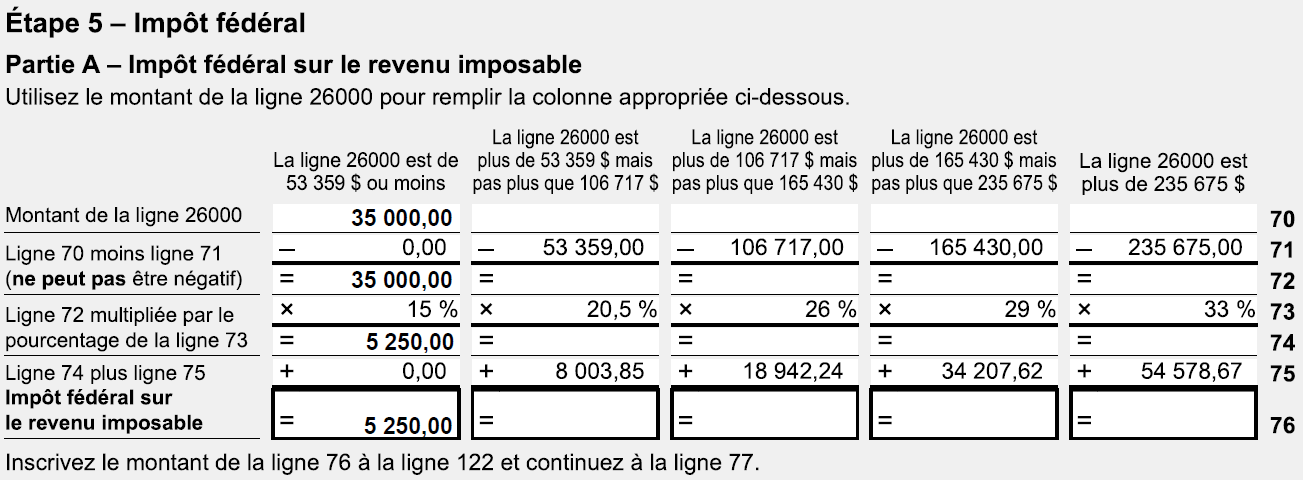
\includegraphics[width=.9\textwidth]{exercice/5-1/Q8/T1-5A.png}
	\caption[]{Exercice 1, T1, partie~A de l'étape 5}
	\label{fig:chap5Exercice1Q8T15A}
\end{figure}

\begin{sousQuestion}
	Calculez le crédit d'impôt pour la contribution politique et le crédit d'impôt relatif aux fonds de travailleurs, puis remplir la partie~C de l'étape 5 de la \href{https://www.canada.ca/fr/agence-revenu/services/formulaires-publications/trousses-impot-toutes-annees-imposition/trousse-generale-impot-prestations/quebec/5005-r.html}{T1} de Michel.
\end{sousQuestion}
L'impôt fédéral de base est de \numprint{5250}~\$ - \numprint{4850}~\$ = 400~\$

La ligne~40900 est de 160~\$, ce qui, avec un crédit de 75~\%, donne 120~\$ à la ligne~41000 pour la contribution politique.

La ligne~41300 est de \numprint{4000}~\$, ce qui, à un taux de crédit de 15~\%, donne 600~\$ à la ligne~41400 pour les fonds de travailleurs.

Le crédit supplémentaire de 720~\$ réduit l'impôt fédéral net à 0~\$, cf. figure~\ref{fig:chap5Exercice1Q8T15C}.
\begin{figure}
	\centering
	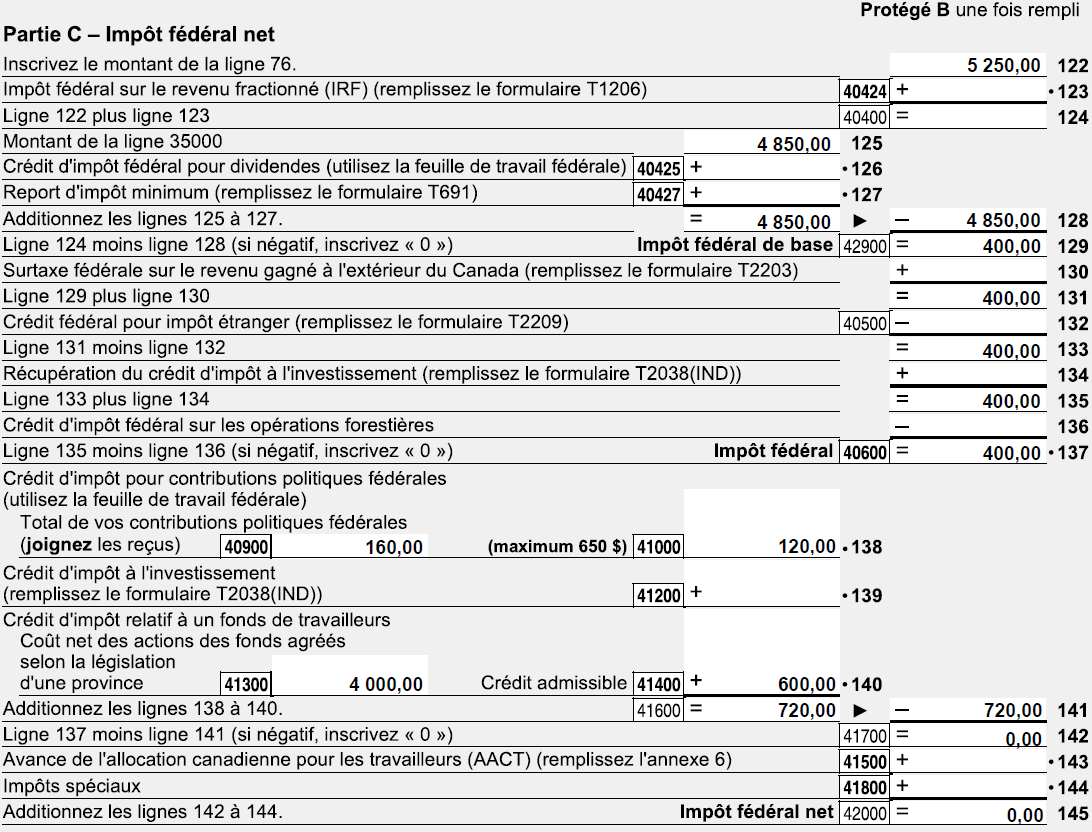
\includegraphics[width=.9\textwidth]{exercice/5-1/Q8/T1-5C.png}
	\caption[]{Exercice 1, T1, partie~C de l'étape 5}
	\label{fig:chap5Exercice1Q8T15C}
\end{figure}

\begin{sousQuestion}
	À la partie~C de l'étape 5, les crédits d'impôts non remboursables sont supérieurs au montant d'impôt à payer. Que peut-il faire avec cette partie inutilisée du crédit d'impôt?
\end{sousQuestion}
Le crédit pour la contribution politique inutilisée ne peut pas être reporté à une année ultérieure. Au fédéral, la contribution versée à un fonds de travailleurs dans la période suivant le 60e jour de l'année d'imposition, c'est-à-dire de mars à décembre~2023, ne peut pas être reportée non plus.

Toutefois, le crédit pour le fonds de travailleurs acheté dans la période des 60 premiers jours de l'année d'imposition suivante, c'est-à-dire janvier et février 2024, peut être reporté sur la déclaration de revenus 2024.

Michel n'a besoin que de 400~\$ de crédits supplémentaires pour réduire son impôt fédéral net à zéro.

Michel peut déclarer comme suit:
\begin{enumerate}
	\item Tout le crédit d'impôt pour la contribution politique de 120~\$ à la ligne~41000;
	\item Le crédit d'impôt au fonds des travailleurs de 300~\$ provenant de sa cotisation de mai~2023.
\end{enumerate}

Il disposera ainsi d'un total de 420~\$ à déclarer à la ligne~41600. Il perdra 20~\$ du crédit de sa contribution de mai~2023, car il ne peut pas la reporter sur sa déclaration fédérale.

Il reportera également une contribution de \numprint{2000}~\$ pour l'année d'imposition 2024.

Il est toujours important de vérifier ce type d'information lorsque vient le temps d'analyser les crédits d'impôt non remboursables d'un contribuable qui réduisent son impôt à payer à zéro.



\section{Calcul de l'impôt du Québec}
\begin{intro}
	Nous avons terminé la discussion sur les crédits non remboursables au chapitre 4 avec le total calculé à la ligne~399.
	
	Dans la partie Impôt sur le revenu et contributions , la première action consiste à calculer l'impôt sur le revenu sur le revenu imposable à l'aide de la grille de calcul 401
\end{intro}
Le principe d'utilisation de la grille de calcul 401 est le même que celui qui est utilisé dans la partie~A de l'étape 5 de  la T1. 



\section{Impôt et cotisations}
\begin{intro}
	Outre la détermination de l'impôt sur le revenu dû, Québec utilise la déclaration de revenus annuelle pour collecter certaines \og contributions \fg{} qui doivent être payées ou des \og avances\fg{} remboursées par le contribuable et qui ne sont pas considérées comme un impôt sur le revenu.
	
	Cette opération s'effectue dans la partie \og Impôt et cotisations \fg{} de la déclaration TP-1. Cette partie~Commence à la page 3 de la TP-1 et se poursuit à la page 4.
\end{intro}

Après avoir déterminé l'impôt à payer sur son revenu imposable à la ligne~401, le contribuable peut demander des crédits d'impôt non remboursables qui vont lui permettre de réduire les impôts qu'il doit payer. Ces crédits d'impôt sont réclamés au bas de la page 3 et comprennent notamment:
\begin{itemize}
	\item Les crédits d'impôt non remboursables, ligne~406 (de la ligne~399);
	\item La contribution aux partis politiques autorisés du Québec, ligne~414;
	\item Le crédit d'impôt pour dividendes, ligne~415, sera étudié au chapitre 6;
	\item Le crédit d'impôt pour actions de Capital régional et coopératif Desjardins, ligne~422;
	\item Le crédit d'impôt relatif à un fonds de travailleurs, ligne~424;
	\item Les crédits non remboursables transférés d'un conjoint à l'autre, ligne~431.
	\item 
\end{itemize}



\section{Contribution politique au Québec}
\index{Contribution politique!Québec}
\begin{intro}
	Un contribuable qui réside au Québec le 31 décembre de l'année d'imposition peut bénéficier d'un crédit d'impôt relativement à une contribution politique.
\end{intro}
Seules les contributions aux partis autorisés au niveau municipal donnent droit au crédit d'impôt sur la déclaration TP-1.

\begin{note}
	La partie inutilisée du crédit ne peut pas être reportée à l'année suivante.
\end{note}



\section{Crédit d'impôt relatif à un fonds de travailleurs - Québec}
Sur la déclaration du Québec, les contribuables peuvent demander un crédit pour les actions achetées durant toute l'année d'imposition et durant les 60 premiers jours de l'année suivante.


\subsection{Exception}
Les règles du Québec pour le report des crédits inutilisés sont plus larges que celles du fédéral.

Si le contribuable n'a pas besoin du montant total du crédit au cours d'une année pour réduire à zéro le montant de la ligne~432 de sa TP-1, contrairement au fédéral, il pourra reporter la partie inutilisée aux années futures.

Si le contribuable a acheté des actions pour un montant supérieur à \numprint{5000}~\$, les crédits associés à l'excédent peuvent également être reportés sur les années suivantes.

Le montant maximal annuel donnant droit au crédit est de \numprint{5000}~\$ pour la totalité des actions acquises du Fondaction et du Fonds de solidarité FTQ. La limite de \numprint{5000}~\$ doit inclure le coût des actions pour lesquelles le crédit d'impôt est reporté des années antérieures.

\begin{rappel}
	En 2021, un changement majeur est intervenu concernant le crédit d'impôt sur les actions de Fondaction. 
	
	Le crédit de 20~\% a été réduit à 15~\% pour tous les achats d'actions de Fondaction effectués après le 31~mai~2021.
\end{rappel}


\subsection{Comment réclamer les crédits}
Au Québec, le crédit d'impôt peut être réclamé à la ligne~424 de la TP-1.

Pour les actions du Fonds de solidarité FTQ, le montant de la case B du relevé 10 (crédit d'impôt) doit être réduit par le crédit d'impôt annulé, inscrit à la case D du feuillet. 

Pour les actions du Fondaction de la CSN, le montant de la case H du relevé 10 doit être réduit par le crédit d'impôt annulé inscrit à la case J du relevé 10. 

Le crédit accordé est le moindre de 750~\$ et de 15~\% du coût net des actions de la FTQ et/ou de Fondaction dont le crédit n'a pas été utilisé l'année précédente et de l'action achetée dans la période en cours. 


\subsection{Autres particularités}
Voici d'autres détails concernant le crédit d'impôt relatif à un fonds de travailleurs:
\begin{itemize}
	\item Si le contribuable utilise un crédit reporté d'une année antérieure, il doit joindre une note expliquant que le relevé 10 a été joint à sa TP-1 de l'année précédente.
	\item Le crédit d'impôt ne peut pas être demandé si les actions ont été achetées pour rembourser des actions rachetées pour participer au Régime d'accession à la propriété ou au Régime d'encouragement à l'éducation permanente d'un REER. 
\end{itemize}



\section{Actions de Capital régional et coopératif Desjardins}
Le crédit que le contribuable peut demander est inscrit à la case B du relevé 26. Il est égal à 30~\% du montant investi (maximum = \numprint{3000}~\$) entre le 1er~mars~2023 et le 28~février~2024. Toute partie du crédit qu'il n'utilise pas dans l'année d'imposition ne peut pas être reportée à une année future. 

\subsection{Crédit d'impôt relatif à l'échange d'actions de Capital régional et coopératif Desjardins}
Un contribuable qui était résident du Québec le 31 décembre de l'année d'imposition peut demander un crédit d'impôt non remboursable pour les actions qu'il a acquises de la nouvelle catégorie d'actions de Capital régional et coopératif Desjardins en échangeant des actions de l'ancienne catégorie qu'il détenait depuis au moins sept ans.

Ce crédit d'impôt non remboursable est accordé pour les années 2019, 2020, 2021, 2022 et 2023. Le taux de crédit d'impôt est égal à 10~\% de la valeur des actions échangées (maximum = \numprint{15000}~\$)



\section{Crédit transféré d'un conjoint à l'autre}
\begin{intro}
	Au Québec, dans leur déclaration de revenus TP-1, les couples peuvent maximiser l'utilisation des crédits non remboursables auxquels ils ont droit.
\end{intro}

Au Québec, il n'y a pas d'équivalent du montant fédéral pour l'époux ou le conjoint de fait sur la déclaration TP-1. Cependant, il existe un mécanisme par lequel les contribuables peuvent transférer à leur conjoint leurs crédits d'impôt non remboursables inutilisés, c'est-à-dire un montant négatif à la ligne~430 de leur TP-1 qu'ils ont et qu'ils perdraient autrement. Ils ne peuvent transférer leurs crédits d'impôt inutilisés à personne d'autre que leur conjoint(e).


\subsection{Conjoint qui a transféré un montant pour enfant majeur aux études postsecondaires}
Il est possible que le conjoint au 31 décembre d'un contribuable ait été aux études en 2023 et qu'il ait transféré, à un de ses parents, un montant pour enfant majeur aux études postsecondaires. Dans une telle situation, si le contribuable désire bénéficier du transfert des crédits inutilisés de son conjoint, il doit réduire le montant négatif, inscrit à la ligne~430 de la TP-1 de son conjoint, d'un montant correspondant à 14~\% du transfert que ce dernier a fait à un de ses parents (ligne~20 de l'annexe~S de votre conjoint).

\rqg{63}



\section{Exercice 2}
\setcounter{question}{0}
\begin{question}
	Durant l'année d'imposition, Rolande a travaillé durant 6 mois dans la province du Nouveau-Brunswick pour deux employeurs différents. À la fin de l'année d'imposition, elle résidait à Trois-Rivières au Québec. Elle a reçu deux T4 indiquant \numprint{1776}~\$ et 692~\$ comme impôts fédéraux retenus à la source. 
	
	Calculez le montant des retenues d'impôt qu'elle peut transférer sur sa déclaration du Québec. Sur quelle ligne de la \href{https://www.canada.ca/fr/agence-revenu/services/formulaires-publications/trousses-impot-toutes-annees-imposition/trousse-generale-impot-prestations/quebec/5005-r.html}{T1} doit-elle réclamer le montant transféré?
\end{question}
Rolande peut transférer \numprint{1110,60}~\$, soit \((\numprint{1776}~\$ + 692~\$) \times 45~\% \) sur sa TP1 à la ligne~454. Le montant est indiqué à la ligne~43800 de sa T1, cf gigure~\ref{fig:chap5Exercice2Q1}.
\begin{figure}
	\centering
	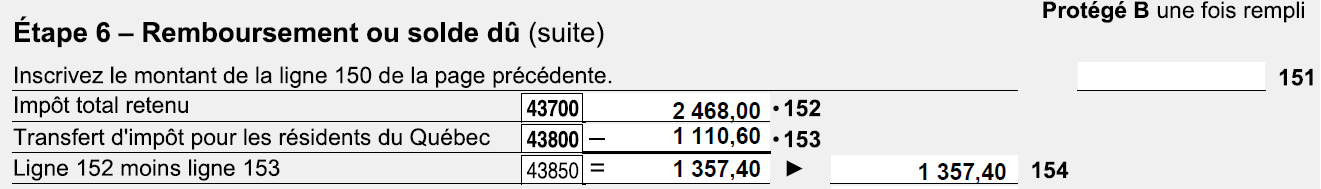
\includegraphics[width=.9\textwidth]{exercice/5-2/Q1/T1-6.png}
	\caption[]{Exercice 2, T1, Transfert d'impôt}
	\label{fig:chap5Exercice2Q1}
\end{figure}

\begin{question}
	Après avoir soustrait le total des crédits remboursables (ligne~48200 de la T1) du total de l'impôt à payer (ligne~43500 de la T1):
\end{question}
\setcounter{sousQuestion}{0}
\begin{sousQuestion}
	Que signifie un montant positif comme réponse?
\end{sousQuestion}
Un solde dû.

\begin{sousQuestion}
	Que signifie un montant négatif comme réponse?
\end{sousQuestion}
Un remboursement.

\begin{question}
	Denis a travaillé pour deux entreprises de sa région durant toute l'année d'imposition. Au fédéral, son impôt fédéral de base et son impôt net sont de \numprint{8520}~\$. Il a également un paiement en trop de 70,50~\$ au RRQ et de 78,74~\$ à l'AE. Le montant total d'impôt retenu à la source est de \numprint{7200}~\$. 
	
	En vous basant sur ces renseignements, complétez la partie \og Remboursement ou solde dû \fg{} de la page 8 de sa \href{https://www.canada.ca/fr/agence-revenu/services/formulaires-publications/trousses-impot-toutes-annees-imposition/trousse-generale-impot-prestations/quebec/5005-r.html}{T1}.
\end{question}
La section \og Remboursement ou solde dû\fg{}, à la page 8 du T1 de Denis est présentée à la figure~\ref{fig:chap5Exercice2Q3}.
\begin{figure}
	\centering
	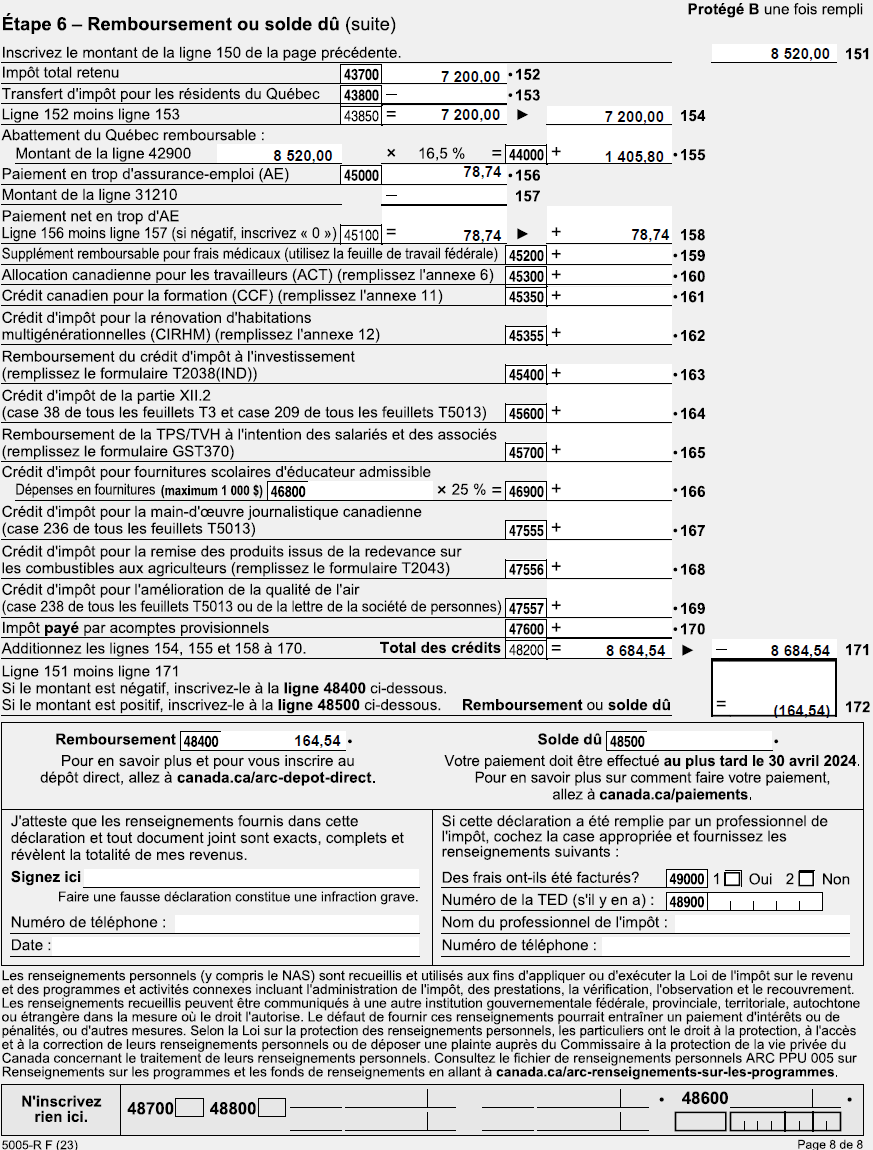
\includegraphics[width=.9\textwidth]{exercice/5-2/Q3/T1-6.png}
	\caption[]{Exercice 2, T1, Remboursement ou solde dû}
	\label{fig:chap5Exercice2Q3}
\end{figure}

NB: Vous devez calculer l'abattement du Québec remboursable et vous rappeler que seul le paiement en trop d'assurance-emploi peut être réclamé sur la T1.

\begin{question}
	Marie donne des cours de création littéraire au Département des études permanentes à l'Université de Montréal. En 2023, elle a payé au total 500~\$ en impressions et photocopies pour lesquelles elle n'a reçu aucun remboursement de la part de l'université.
	
	Marie peut-elle réclamer le crédit d'impôt pour fournitures scolaires des enseignants à l'égard de ses dépenses?
\end{question}
Non, Marie ne peut pas réclamer le crédit d'impôt pour fournitures scolaires des enseignants à l'égard de ses dépenses car elle est enseignante dans une université. Marie doit enseigner dans une école primaire ou secondaire pour être admissible à ce crédit.

\begin{question}
	Laquelle des dépenses suivantes ne serait pas admissible au crédit d'impôt pour fournitures scolaires des enseignants, si la dépense est faite par un enseignant du primaire?
	\begin{enumerate}[label=\Alph*.]
		\item Livres à colorier et crayons de couleur
		\item Les billets d'autobus pour amener les enfants à une foire scientifique
		\item Jeux d'échecs et damiers
	\end{enumerate}
\end{question}
B. Les billets d'autobus pour amener les enfants à une foire scientifique.



\section{Versement anticipé et cotisation payable}
\begin{intro}
	Outre la détermination de l'impôt sur le revenu dû, Québec utilise la déclaration de revenus annuelle pour collecter certaines \og contributions \fg{} qui doivent être payées ou des \og avances\fg{} remboursées par le contribuable et qui ne sont pas considérées comme un impôt sur le revenu.
	
	Par conséquent, ces contributions sont ajoutées à l'impôt sur le revenu dû.
\end{intro}

Après avoir réduit son impôt à payer avec les crédits d'impôt non remboursables, l'impôt \textbf{}restant à payer est inscrit à la ligne~432 au bas de la page 3 et en haut de la page 4. 

La liste suivante identifie les contributions qui seront ou vont été discutées dans ce cours:
\begin{itemize}
	\item À la ligne~439, la cotisation au RQAP pour un travail hors du Québec.
	\item Si nécessaire, revoyez la discussion relative au RQAP au chapitre 3;
	\item À la ligne~441, le contribuable doit inscrire tous les versements anticipés reçus pour les crédits d'impôt relatifs à la prime au travail, pour le maintien à domicile des aînés, pour les frais de garde d'enfants et pour le traitement de l'infertilité. Les montants figurent sur le relevé 19 (présentés dans les chapitres 7 à 12);
	\item À la ligne~446, la cotisation au Fonds des services de santé (voir chapitre 6);
	\item À la ligne~447, la cotisation au Régime d'assurance médicaments du Québec (RAMQ).
\end{itemize}



\section{Régime d'assurance médicaments du Québec}
\begin{intro}
	La Régie de l'assurance maladie du Québec (RAMQ) est le régime public d'assurance maladie du Québec, qui permet à \textbf{tous les résidents du Québec d'avoir accès à des soins de santé gratuits}.
	
	Une partie des soins de santé est le régime public d'assurance-médicaments pour lequel les contribuables, en fonction de leur situation familiale, peuvent être amenés à contribuer au financement par le biais du paiement d'une prime.
	
	Dans cette section, nous discutons de la question de savoir qui doit payer une telle prime et quel est le montant de la prime à payer.
\end{intro}
Si en 2023, le contribuable possédait une carte d'assurance-maladie émise par la Régie de l'assurance maladie du Québec (RAMQ), il devait être couvert par:
\begin{itemize}
	\item Un régime d'assurance collective qui offre une assurance médicaments de base; ou
	\item Le régime d'assurance médicaments du Québec, qui est un \og régime public \fg{} de la Régie de l'assurance maladie du Québec.
\end{itemize}

\index{Régime privé}
La RAMQ utilise le terme \textbf{régime privé} pour désigner un régime d'assurance collective afin de le différencier du Régime d'assurance-médicaments du Québec. 


\subsection{Régimes privés}
Un contribuable peut avoir accès à un régime privé de deux façons:
\begin{enumerate}
	\item \textbf{Dans le cadre de son emploi ou de sa profession.} En effet, plusieurs employeurs offrent à leur personnel la possibilité d'adhérer à un régime privé. Il en est de même des associations et ordres professionnels qui proposent ce genre de régime à leurs membres.
	
	La plupart du temps, la protection pour les médicaments est incluse dans un régime couvrant d'autres soins de santé (appelé régime d'assurance maladie). Parfois, cette protection est offerte seule.
	\item \textbf{Par l'intermédiaire de son/sa conjoint(e) ou de ses parents.} Les personnes qui ont accès à un régime privé doivent y adhérer. De plus, elles sont obligées de couvrir leur conjoint et leurs enfants, sauf si ceux-ci bénéficient d'une telle couverture d'un autre régime privé.
\end{enumerate}

En règle générale, la prime payée par l'employeur au nom de l'employé est considérée comme un avantage imposable pour les employés travaillant au Québec. Cet avantage est indiqué à la case J ou P du Relevé1 et est inclus dans le montant de la case A. Lorsqu'un montant est inscrit à la case P, le contribuable doit recevoir un Relevé 22.


\subsection{Régime public}
Une personne doit s'inscrire au régime public lorsqu'elle cesse d'être admissible à un régime privé. Pour être admissible au régime public, le contribuable doit résider au Québec et être inscrit au régime. Pour être admissible au régime public:
\begin{itemize}[label=\twemoji{check mark button}]
	\item Le contribuable de 18 à 64 ans qui n'a pas accès à un régime privé;
	\item Le contribuable de 65 ans ou plus. Lorsqu'il atteint 65 ans, le contribuable est automatiquement inscrit au régime public. Toutefois, il peut choisir de continuer à être couvert par un régime privé. S'il choisit de demeurer dans le régime privé, il doit annuler son inscription au régime public;
	\item Le prestataire de l'assistance sociale ou le prestataire du Programme objectif emploi et celui détenteur d'un carnet de réclamation;
	\item Les enfants du contribuable assuré par ce régime.
\end{itemize}

Le contribuable assuré par le régime public doit en principe participer au financement du régime d'assurance médicaments du Québec de deux façons:
\begin{itemize}
	\item En payant une franchise et une coassurance à l'achat de médicaments;
	\item En payant une cotisation (prime) au régime d'assurance médicaments du Québec lorsqu'il produit sa déclaration de revenus du Québec. Pour 2023, la cotisation varie de 0~\$ à 720,50~\$ par adulte.
\end{itemize}

\begin{note}
	Le contribuable doit payer une cotisation au régime d'assurance médicaments du Québec s'il était couvert par une assurance qui n'offre pas une couverture de base pour ses médicaments (c'est-à-dire une couverture équivalente à celle offerte par la RAMQ).
\end{note}


\subsection{Calcul de la cotisation au Régime d'assurance médicaments du Québec}
Le contribuable doit utiliser l'annexe~K, Cotisation au régime d'assurance médicaments du Québec, afin de calculer la cotisation qu'il doit verser à la RAMQ.

\begin{note}
	Si le contribuable ou son conjoint a un régime privé, il inscrira à la case 449 l'un des codes suivants:
	\begin{itemize}
		\item \og 14 \fg{} en tant que membre du régime privé d'assurance collective; ou
		\item \og 16 \fg{} puisque son conjoint ou parent (père / mère) était membre du régime privé d'assurance collective.
	\end{itemize}
	
	Si le contribuable a fourni les informations requises sur son conjoint dans la section 2 de la partie~B, de l'annexe~K et a choisi de payer la prime de son conjoint, ce dernier doit inscrire \og 20 \fg{} à la case 449.
\end{note}

\begin{note}
	Le contribuable qui reçoit un supplément de revenu garanti (SRG) (dont il sera question dans le chapitre 10) peut être exempté du paiement de la cotisation. Cette exonération est \textbf{conditionnelle} à l'état civil du contribuable, son âge à la fin de l'année, si la somme reçue mensuellement à titre de supplément de revenu garanti (SRG) dépasse le seuil donné et s'ils ont reçu des médicaments gratuits \textbf{tout au long} de 2023 en raison du montant du SRG reçu.
\end{note}

\subsubsection{partie~A de l'annexe~K}
Un \og enfant à charge \fg{} aux lignes~42 et 44 de l'annexe~K, désigne une personne pour qui le contribuable ou son conjoint au 31 décembre:
\begin{itemize}
	\item A reçu un paiement d'allocation famille en 2023;
	\item Inscrit un montant transféré par un enfant majeur aux études postsecondaires à la ligne~28 de leur annexe~A.
\end{itemize}

\subsubsection{partie~B de l'annexe~K}
La partie \og 2 - Votre conjoint \fg{} ne doit être remplie que si le contribuable choisit de payer la prime de son conjoint. Le conjoint n'a pas à remplir l'annexe~K et inscrit simplement \og 20 \fg{} à la case 449 de sa déclaration TP-1.

\paragraph{Nombre de mois pour lesquels la prime n'est pas due}
La partie~B comprend une série de situations dans lesquelles le contribuable n'est pas tenu de payer la prime pour un mois donné.

Notez les points suivants:
\begin{itemize}
	\item Le contribuable, auquel l'une de ces situations s'applique même pour un seul jour d'un mois donné, coche le mois en question;
	\item Le contribuable et son conjoint peuvent se trouver dans des situations différentes;
	\item Un étudiant célibataire à temps plein âgé de 18 à 25 ans qui ne vit pas avec ses parents doit payer une prime au régime s'il n'est pas couvert par un régime privé;
	\item Les personnes qui étaient en centre d'hébergement et de soins de longue durée (CHSLD) ne paient pas de prime. Le CHSLD assume le coût des médicaments;
	\item Les ressortissants étrangers, les résidents d'une autre province qui ont exploité une entreprise au Québec et les contribuables qui sont restés à l'extérieur du Québec pendant toute l'année ne paient pas de prime;
	\item Si les contribuables ont déménagé du Québec au cours de l'année et qu'ils n'ont pas bénéficié d'une couverture privée pour les mois où ils ont vécu au Québec, ils doivent remplir un TP-1 pour payer une prime. Revenu Québec conseille au contribuable de le contacter.
\end{itemize}

\begin{note}
	Pour toutes les situations énumérées dans la partie~B, il est important de consulter le guide de la déclaration TP-1 concernant la ligne~447.
\end{note}

\subsubsection{partie~C de l'annexe~K}
La partie~C permet au contribuable d'établir le montant de la cotisation qu'il doit payer.

La cotisation de la RAMQ peut être réclamée comme frais médical sur la T1 pour l'année d'imposition où elle a été payée. Sur la TP-1, même si elle a été payée dans l'année suivant l'année d'imposition, elle est considérée avoir été payée le 31 décembre de l'année d'imposition. 

\rqg[s]{67-70}



\section{Calcul du Remboursement ou solde à payer - Québec}
\begin{intro}
	La partie \og Impôt et cotisations \fg{} aux pages 3 et 4 de la TP-1 permet au contribuable de déterminer le montant qu'il doit à Revenu Québec.
	
	Après avoir déterminé ses impôt et cotisations, le contribuable doit établir les crédits d'impôt remboursables auxquels il a droit. Pour les réclamer, il doit se servir de la partie \og Remboursement ou solde à payer \fg{} de la TP-1.
\end{intro}

Pour clore ce chapitre et arriver enfin au résultat d'un remboursement ou d'un solde dû, nous aborderons les crédits d'impôt remboursables suivants:
\begin{itemize}
	\item Impôt du Québec retenu à la source;
	\item La cotisation payée en trop au RRQ;
	\item Portion de l'impôt retenu par une autre province transférée au Québec;
	\item La cotisation payée en trop au RQAP.
\end{itemize}

Voici les crédits d'impôt remboursables qui seront discutés dans les chapitres 7 à 12:
\begin{itemize}
	\item Remboursement de l'impôt du Québec transféré à ou par votre conjoint;
	\item L'impôt payé par acomptes provisionnels;
	\item Les frais de garde d'enfants;
	\item La prime au travail;
	\item Le maintien à domicile des aînés;
	\item Le Bouclier fiscal;
	\item Soutien aux aînés;
	\item Compensation financière pour maintien à domicile;
	\item Les crédits d'impôt remboursables qui sont inclus à la ligne~462, notamment:
	\begin{itemize}
		\item Les frais médicaux;
		\item Personne aidante;
		\item Frais d'adoption;
		\item Remboursement de prestations;
		\item Traitement de l'infertilité;
		\item Athlète de haut niveau;
		\item Frais engagés par un aîné pour maintenir son autonomie;
		\item Activités des enfants;
		\item Subvention pour aînés relative à une hausse de taxes municipales;
		\item Mise aux normes d'installations d'assainissement des eaux usées résidentielles.
	\end{itemize}
\end{itemize}

\subsection{Impôt du Québec retenu à la source}
Le contribuable doit inscrire à la ligne~451 de sa TP-1 la totalité de l'impôt provincial retenu à la source, qui est inscrit sur ses relevés ou feuillets de renseignements. 

\subsection{Partie transférable de l'impôt retenu pour une autre province}
Comme mentionné au début de ce chapitre, le montant maximum transférable correspond à 45~\% du total de l'impôt payé hors du Québec. Le montant transféré doit être inscrit à la ligne~454 de la TP-1. 

\subsection{Cotisations payées en trop au RRQ/RQAP}
Comme nous l'avons vu au chapitre 3, tout paiement excédentaire effectué par le contribuable au RRQ et au RQAP est remboursé aux lignes~452 et 457 respectivement.

\subsection{Impôt et cotisations versus, impôt payé et autres crédits remboursables}
Si le résultat de la ligne~470 est positif, le contribuable a un solde à payer à la ligne~475.

Ce montant est payable au plus tard le 30 avril suivant la fin de l'année d'imposition. Après cette date, des intérêts seront exigibles jusqu'à la date du paiement final du solde.

\subsection{Remboursement transféré au conjoint}
Un contribuable ayant droit à un remboursement peut demander à Revenu Québec de transférer tout ou partie de son remboursement à son conjoint, si ce dernier a un solde dû.

Si le contribuable opte pour cette solution, aucune modification n'est possible une fois que la déclaration TP-1 a été produite.

Le montant qui peut effectivement être transféré est celui calculé selon l'avis de cotisation du Québec.

\subsection{Remboursement anticipé}
Un contribuable peut demander de recevoir son remboursement avant même que sa déclaration TP-1 soit traitée. Pour demander le remboursement anticipé, il doit remplir toutes les conditions suivantes de Revenu Québec:
\begin{itemize}
	\item Il demande un remboursement de \numprint{3000}~\$ ou moins à la ligne~474;
	\item Il a produit une déclaration de revenus pour l'année d'imposition 2022;
	\item Il n'a pas changé de nom ni de numéro d'assurance sociale;
	\item Il n'a aucune dette envers Revenu Québec ou tout autre organisme gouvernemental de niveau provincial;
	\item Il n'a pas fait faillite l'année 2022;
	\item Il n'inscrit aucun montant à la ligne~476;
	\item Il produit sa TP-1 pour 2023 avant le 1er mai 2024, ou avant le 18 juin 2024 si lui ou son conjoint déclare un revenu d'entreprise.
\end{itemize}

\subsection{Dépôt direct}
Un contribuable peut s'inscrire au \og Dépôt direct \fg{} pour le remboursement d'impôt du Québec de trois façons, soit:
\begin{itemize}[label=\twemoji{check box with check}]
	\item En faisant une \href{https://www.revenuquebec.ca/fr/citoyens/votre-situation/depot-direct/}{demande en ligne} à partir du site Internet de Revenu Québec;
	\item En attachant à la page 1 de sa déclaration TP-1 un spécimen de chèque portant la mention \og ANNULÉ \fg{} au recto, ainsi que ses nom et numéro d'assurance sociale;
	\item En remplissant le formulaire \href{https://www.revenuquebec.ca/fr/services-en-ligne/formulaires-et-publications/details-courant/lm-3/}{LM-3 -- Demande d'inscription au dépôt direct}, et en l'attachant à la page 1 de sa déclaration TP-1.
\end{itemize}

\subsection{Solde à payer}
Le contribuable a plusieurs possibilités pour payer son solde. Il peut faire le paiement par chèque ou mandat à l'ordre du ministre du Revenu du Québec. Il doit alors remplir le formulaire \textbf{TPF-1026.0.2, Bordereau de paiement}, qui est fourni dans le cahier \og Formulaire \fg{} et l'attacher, avec le chèque ou mandat, à la page 1 de sa déclaration. Il peut aussi faire le paiement au comptoir d'une institution financière, en utilisant le Bordereau de paiement (TPF-1026.0.2). Enfin, il peut acquitter son solde à payer par Internet.

\section{Exercice 3}
\setcounter{question}{0}
\begin{question}
	Au Québec, calculez l'impôt sur le revenu imposable de Arthur et de Mélanie.
	
	\href{https://www.revenuquebec.ca/documents/fr/formulaires/tp/2023-12/TP-1.D.GR%282023-12%29.pdf}{Grilles de calcul} (401).
\end{question}
\setcounter{sousQuestion}{0}
\begin{sousQuestion}
	Arthur: \numprint{51360}~\$
\end{sousQuestion}
Grille de calcul 401 pour calculer le revenu imposable d'Arthur: figure~\ref{fig:chap5Exercice3Q1a}.
\begin{figure}
	\centering
	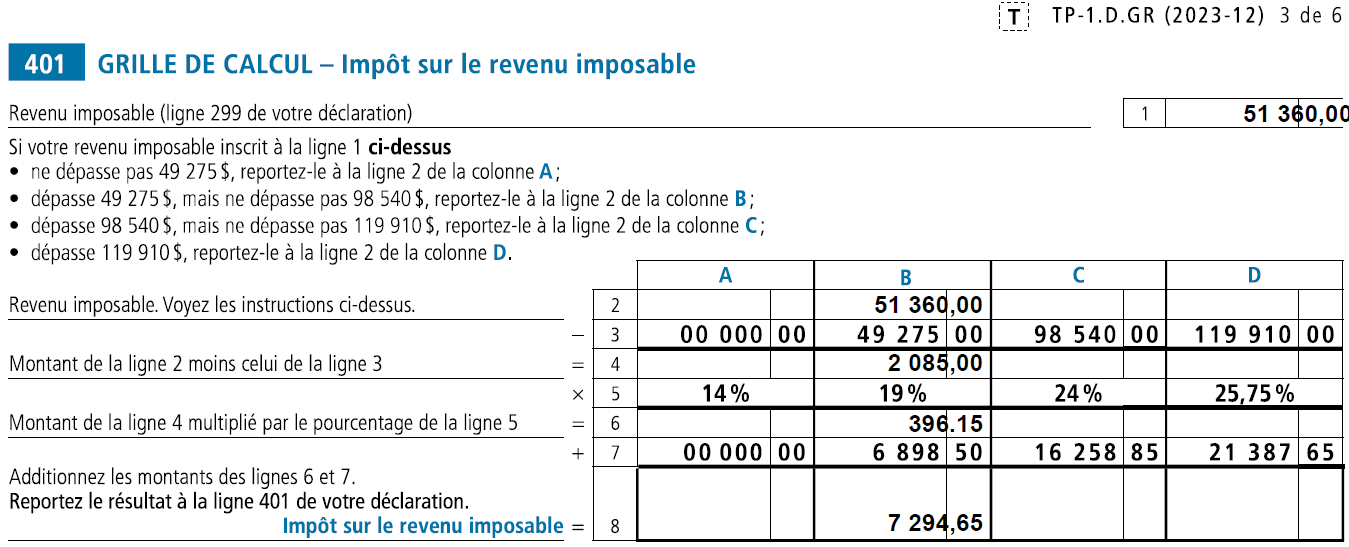
\includegraphics[width=.9\textwidth]{exercice/5-3/Q1/TP1-401-Arthur.png}
	\caption[]{Exercice 3, TP-1, Impôt sur le revenu imposable}
	\label{fig:chap5Exercice3Q1a}
\end{figure}

\begin{sousQuestion}
	Mélanie: \numprint{115655}~\$
\end{sousQuestion}
Grille de calcul 401 pour calculer le revenu imposable de Mélanie: figure~\ref{fig:chap5Exercice3Q1b}.
\begin{figure}
	\centering
	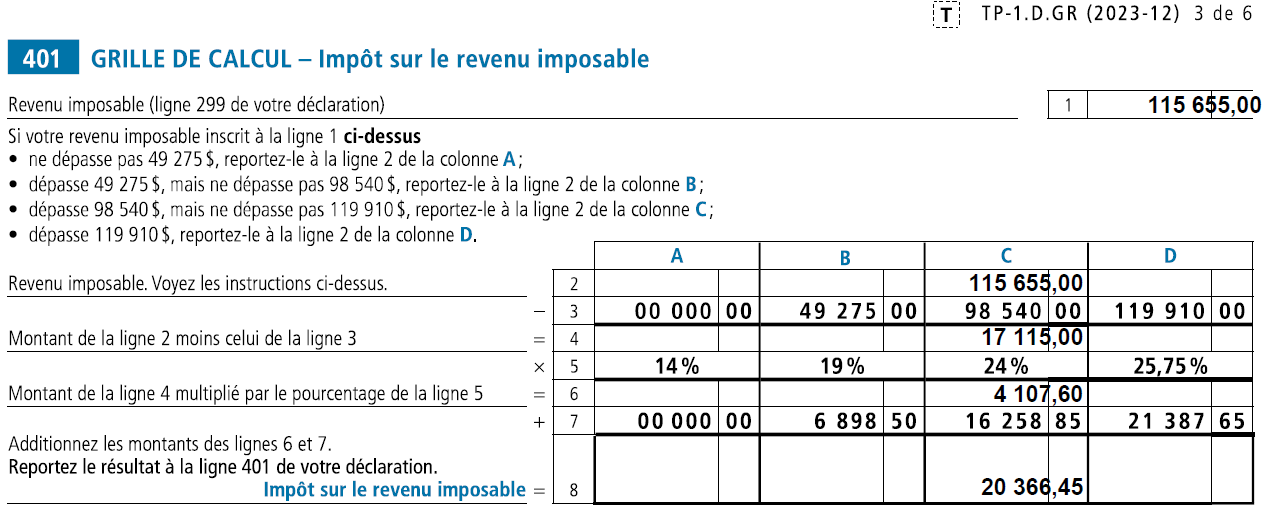
\includegraphics[width=.9\textwidth]{exercice/5-3/Q1/TP1-401-Melanie.png}
	\caption[]{Exercice 3, TP-1, Impôt sur le revenu imposable (bis)}
	\label{fig:chap5Exercice3Q1b}
\end{figure}

\begin{question}
	Durant l'année d'imposition, Madeleine a versé 500~\$ au Parti libéral fédéral, 500~\$ au Parti libéral provincial et 280~\$ à un parti municipal autorisé au Québec. 
	
	Calculez le crédit d'impôt pour les contributions politiques qu'elle peut réclamer sur sa déclaration TP-1.
	
	\href{https://www.revenuquebec.ca/documents/fr/formulaires/tp/2023-12/TP-1.D.GR%282023-12%29.pdf}{Grilles de calcul} (414).
\end{question}
Sur sa TP-1, Madeleine peut réclamer seulement la contribution versée à un parti municipal (maximum 200~\$). Elle ne peut pas réclamer ni reporter la partie non utilisée de 80~\$.

Madeleine pourra réclamer le crédit pour la contribution de 500~\$ pour un parti politique fédéral sur sa T1. Elle ne peut réclamer le montant versé au Parti libéral du Québec.

\begin{question}
	Pour des actions acquises d'un fonds de travailleurs du Québec, quelle est la principale différence entre le crédit d'impôt fédéral et le crédit d'impôt provincial relatif à un fonds de travailleurs?
\end{question}
Au Québec, il est possible de reporter la partie inutilisée du crédit d'impôt qui n'est pas utilisée pour l'année d'imposition courante aux années suivantes, peu importe à quel moment les actions ont été acquises.

Au fédéral, il est possible de reporter à l'année d'imposition suivante (2024) seulement la partie du crédit relatif aux actions acquises dans les 60 premiers jours de l'année 2024.

\begin{question}
	Martha Choquette, dont le NAS est 800 001 240, est née le 10 septembre 1976 (47 ans). Elle est célibataire et n'a aucune personne à charge. Elle a droit au montant pour personne vivant seule.
	
	Durant les mois de janvier à avril, elle a reçu des prestations d'assistance sociale. Elle a recommencé à travailler le 1er mai. Elle n'a bénéficié d'aucune protection de son employeur, relativement à une assurance médicaments. Le montant inscrit aux lignes~275 et 299 de sa TP-1 est de \numprint{19940}~\$.
	
	Établissez le montant de la cotisation au Régime d'assurance médicaments du Québec de Martha à l'aide de l'annexe~K, qui est présentée ci-dessous. 
\end{question}
annexe~K, page 1: Figure~\ref{fig:chap5Exercice3Q4K1}

annexe~K, page 2: Figure~\ref{fig:chap5Exercice3Q4K2}
\begin{figure}
	\centering
	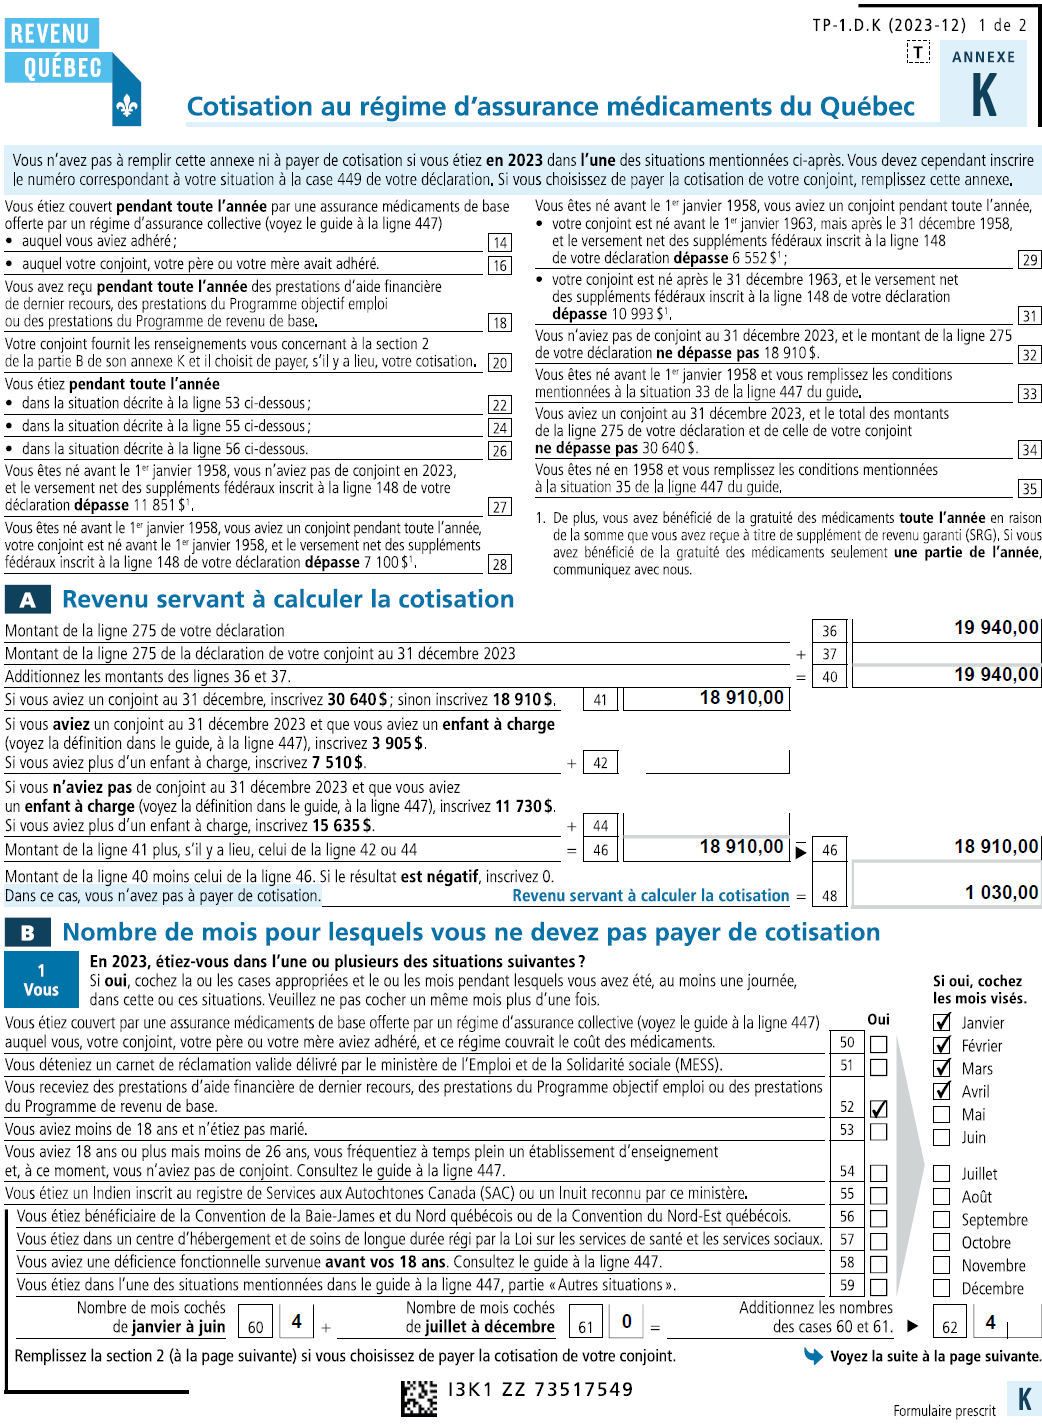
\includegraphics[width=.9\textwidth]{exercice/5-3/Q4/AnnexeK-page1.png}
	\caption[]{Exercice 3, TP-1, annexe~K, page 1}
	\label{fig:chap5Exercice3Q4K1}
\end{figure}
\begin{figure}
	\centering
	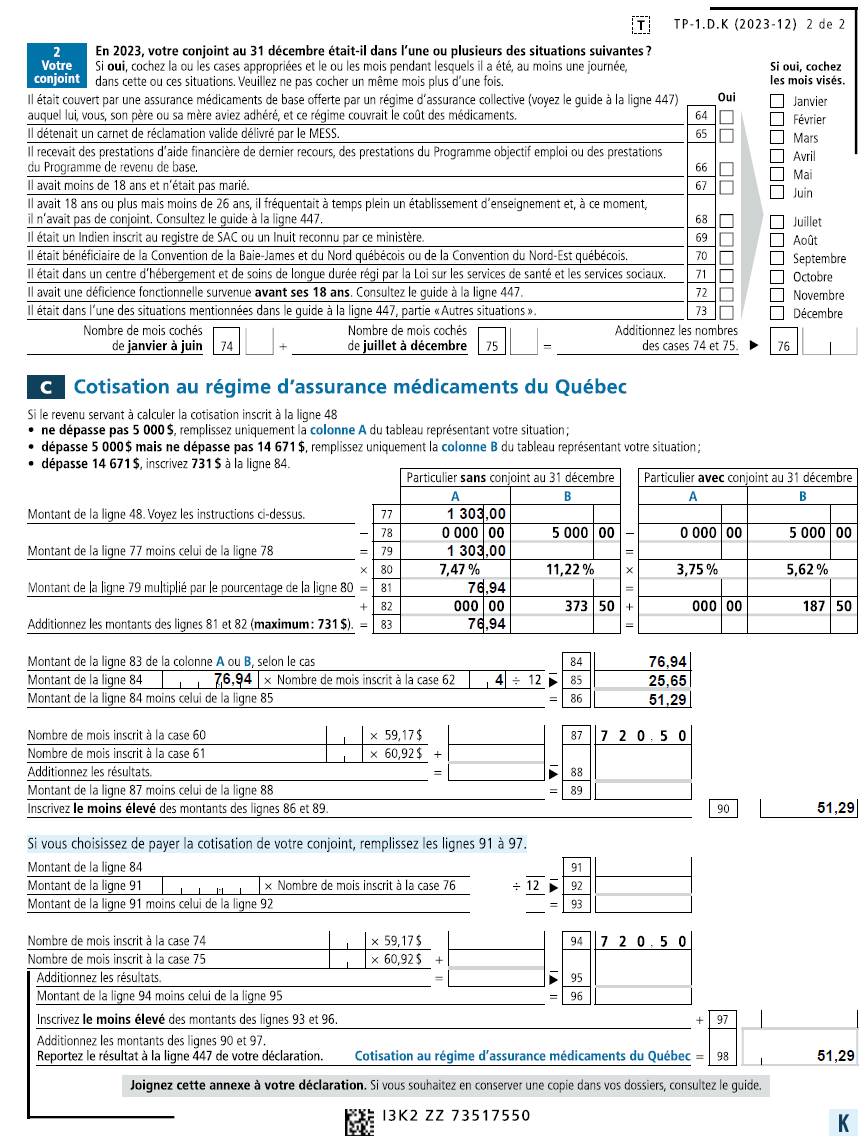
\includegraphics[width=.9\textwidth]{exercice/5-3/Q4/AnnexeK-page2.png}
	\caption[]{Exercice 3, TP-1, annexe~K, page 2}
	\label{fig:chap5Exercice3Q4K2}
\end{figure}
\begin{question}
	Le 2~mars~2023, Frank a contribué \numprint{2200}~\$ au FTQ. Le 15~septembre~2023, il a contribué \numprint{1200}~\$ au Fondaction.
	
	Au Québec, quel est le crédit d'impôt maximal que Frank peut réclamer relativement à ces deux fonds de travailleurs? Montrez vos calculs.
\end{question}
Au cours des années précédentes, le taux de crédit pour les actions de Fondaction était différent de celui des actions de la FTQ.

Aujourd'hui, les taux de crédit sont tous deux de 15 %.

Le crédit est donc de 15~\% de \numprint{3400}~\$ ( \numprint{2200}~\$ + \numprint{1200}~\$) = 510~\$

\section{Sommaire du chapitre}
\begin{itemize}[label=\twemoji{star}]
	\item Le crédit d'impôt pour les contributions politiques diffère au niveau fédéral et au Québec.
	\item Les crédits d'impôt relatifs à un fonds de travailleurs sont à 15~\% tant au fédéral qu'au Québec depuis le 1er juin 2021.
	\item Les crédits d'impôts non remboursables au Québec comme au fédéral ne sont tout simplement pas remboursables lorsque l'impôt à payer est réduit à 0~\$. Toutefois, au Québec, si vous avez un conjoint, vous pouvez lui transférer les crédits d'impôt restants après la mise à zéro de l'impôt à payer.
	\item Au Québec, le contribuable n'ayant pas de régime privé d'assurance-médicaments est dans l'obligation de payer une cotisation au régime public, soit la RAMQ. Certains contribuables peuvent en être exemptés.
\end{itemize}



\section{Problème de révision}
\subsection{Renseignements du contribuable}
Voir la table \ref{table:chapitre5ProblemeRenseignementsContribuable}.
\begin{table}
	\centering
	\begin{tabular}{|l|c|}
		\hline
		\rowcolor{LightGreen} Description        &      Contribuable      \\ \hline
		Nom                                      &   Wâpaskw Mestokosho   \\ \hline
		NAS                                      &      801 115 510       \\ \hline
		Date de naissance                        &    18 janvier 1970     \\ \hline
		Statut civil                             &          Veuf          \\ \hline
		Sexe                                     &           M            \\ \hline
		Province de résidence                    &           QC           \\ \hline
		Langue                                   &           A            \\ \hline
		Téléphone                                &      418-345-3608      \\ \hline
		Adresse courriel                         & w.mestokosho@gmail.com \\ \hline
		Consentement à l'envoi de communications &          Oui           \\
		par voie électronique uniquement         &                        \\ \hline
		Régime d'assurance médicaments           &          RAMQ          \\ \hline
		Adresse                                  &  337 rue Des Érables,  \\
		                                         & Sept-Îles, QC, G0W 1H0 \\ \hline
		Citoyenneté canadienne                   &          Oui           \\ \hline
		Élections Canada                         &          Oui           \\ \hline
		Biens étrangers                          &          Non           \\ \hline
		Revenu                                   &          Oui           \\ \hline
	\end{tabular}
	\caption[]{Problème, renseignements du contribuable}
	\label{table:chapitre5ProblemeRenseignementsContribuable}
\end{table}


\subsection{Renseignements sur les personnes à charge}
Voir la table \ref{table:chapitre5ProblemeRenseignementsPersonnesACharge}.
\begin{table}
	\centering
	\begin{tabular}{|l|c|c|}
		\hline
		\rowcolor{LightGreen} Description & Personne à charge 1 & Personne à charge 2 \\ \hline
		Nom                               & Âpikusîs Mestokosho & Wîskacân Mestokosho \\ \hline
		Lien                              &        Fille        &        Fils         \\ \hline
		NAS                               &     801 115 528     &     801 115 536     \\ \hline
		Date de naissance                 &     10 mai 2006     &     2 mars 2002     \\ \hline
	\end{tabular}
	\caption[]{Problème, renseignements sur les personnes à charge}
	\label{table:chapitre5ProblemeRenseignementsPersonnesACharge}
\end{table}


\subsection{Informations supplémentaires de Wâpaskw}
\begin{itemize}
	\item Wâpaskw vit seul avec ses deux enfants.
	\item Il a un reçu pour une contribution de 500~\$ au parti politique fédéral Nouveau Parti Démocratique.
	\item Il a aussi un reçu pour une contribution de 500~\$ à un parti politique municipal.
	\item Wâpaskws'est procuré des actions de Fondaction et du FTQ.
	\item Wâpaskw est inscrit au dépôt direct.
	\item La déduction bonifiée du RRQ de Wâpaskw est de 473,03~\$
\end{itemize}


\subsection{Informations supplémentaires sur les personnes à charge}
\begin{itemize}
	\item Âpikusîs souffre d'une mobilité réduite. Elle a une attestation écrite de son médecin.
	\item Son revenu net de \numprint{1550}~\$ tant au fédéral qu'au Québec.
	\item Wîskacân poursuit des études postsecondaires au CEGEP. Il a reçu un Relevé 8 pour ses études.
	\item Il tient à transférer le montant pour enfant majeur aux études postsecondaires à son père.
	\item Wîskacân a reçu quatre versements du crédit de solidarité totalisant 305~\$.
	\item Son revenu net de \numprint{2200}~\$ tant au Québec qu'au fédéral.
\end{itemize}


\subsection{Feuillets de Wâpaskw}
\begin{description}
	\item[RL-31] Figure \ref{fig:chap5ProblemeRL31}
	\item[T4] Figure \ref{fig:chap5ProblemeT4}
	\item[RL-1] Figure \ref{fig:chap5ProblemeRL1}
	\item[RL-10 FTQ] Figure \ref{fig:chap5ProblemeRL10FTQ}
	\item[RL-10 Fondaction] Figure \ref{fig:chap5ProblemeRL10Fondaction}
\end{description}

\begin{figure}
	\centering
	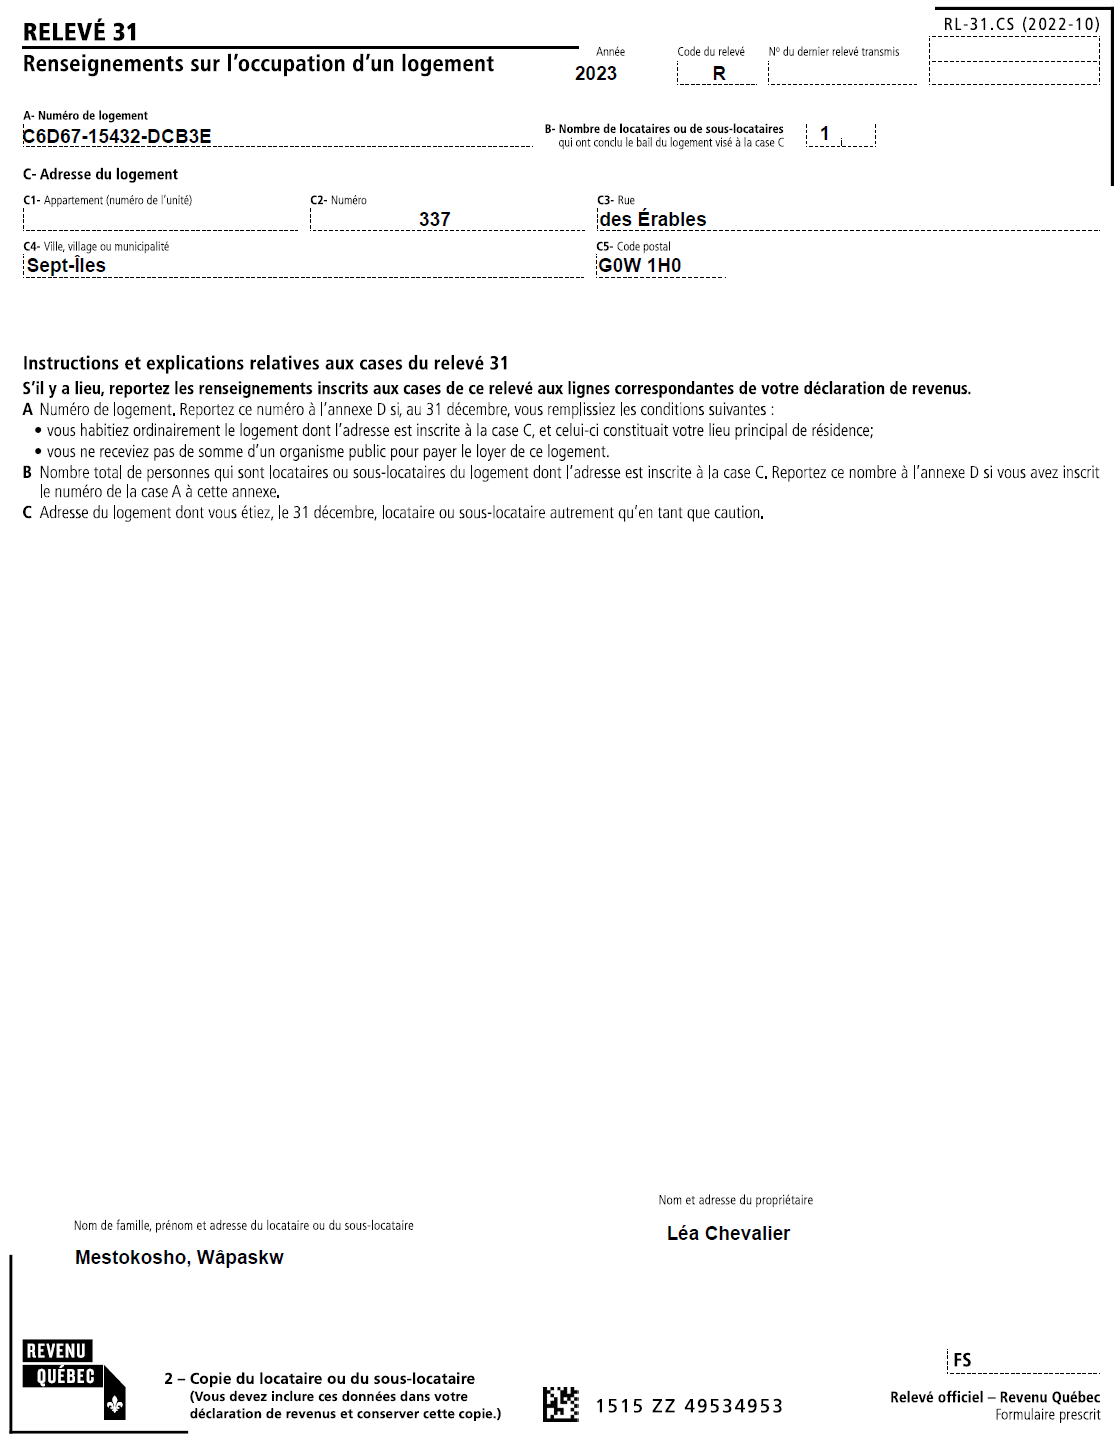
\includegraphics[width=.9\textwidth]{probleme/chapitre-5/Wapaskw-RL31.png}
	\caption[]{Problème, RL-31}
	\label{fig:chap5ProblemeRL31}
\end{figure}
\begin{figure}
	\centering
	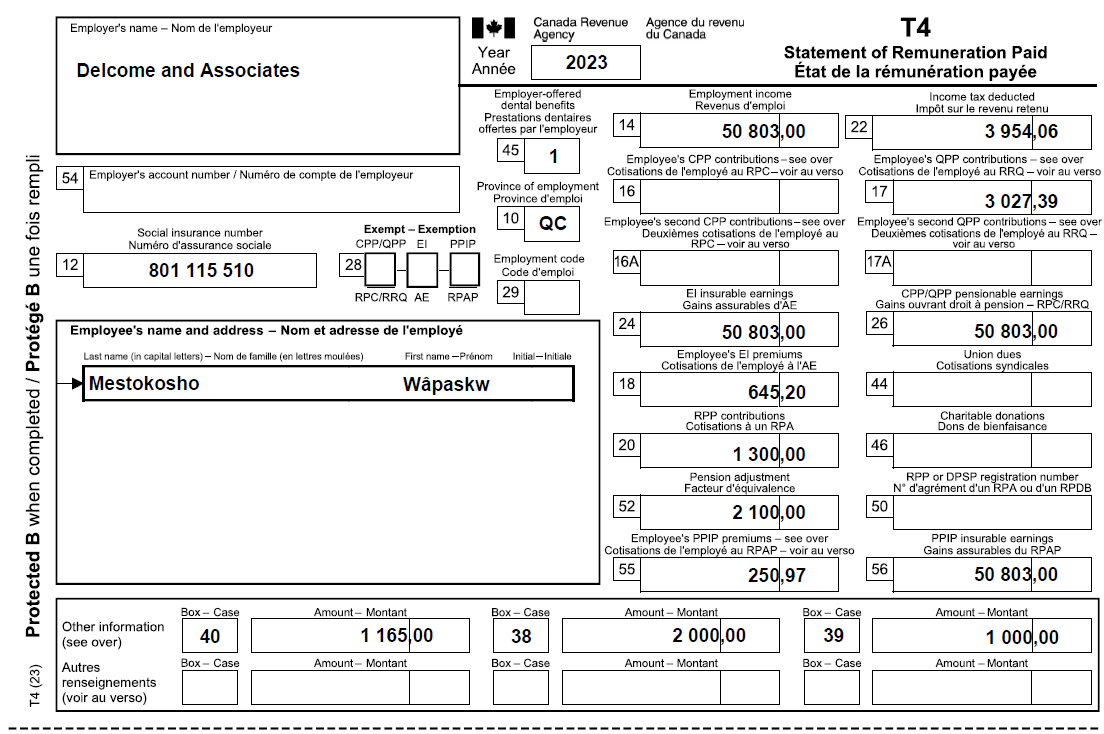
\includegraphics[width=.9\textwidth]{probleme/chapitre-5/Wapaskw-T4.png}
	\caption[]{Problème, T4}
	\label{fig:chap5ProblemeT4}
\end{figure}
\begin{figure}
	\centering
	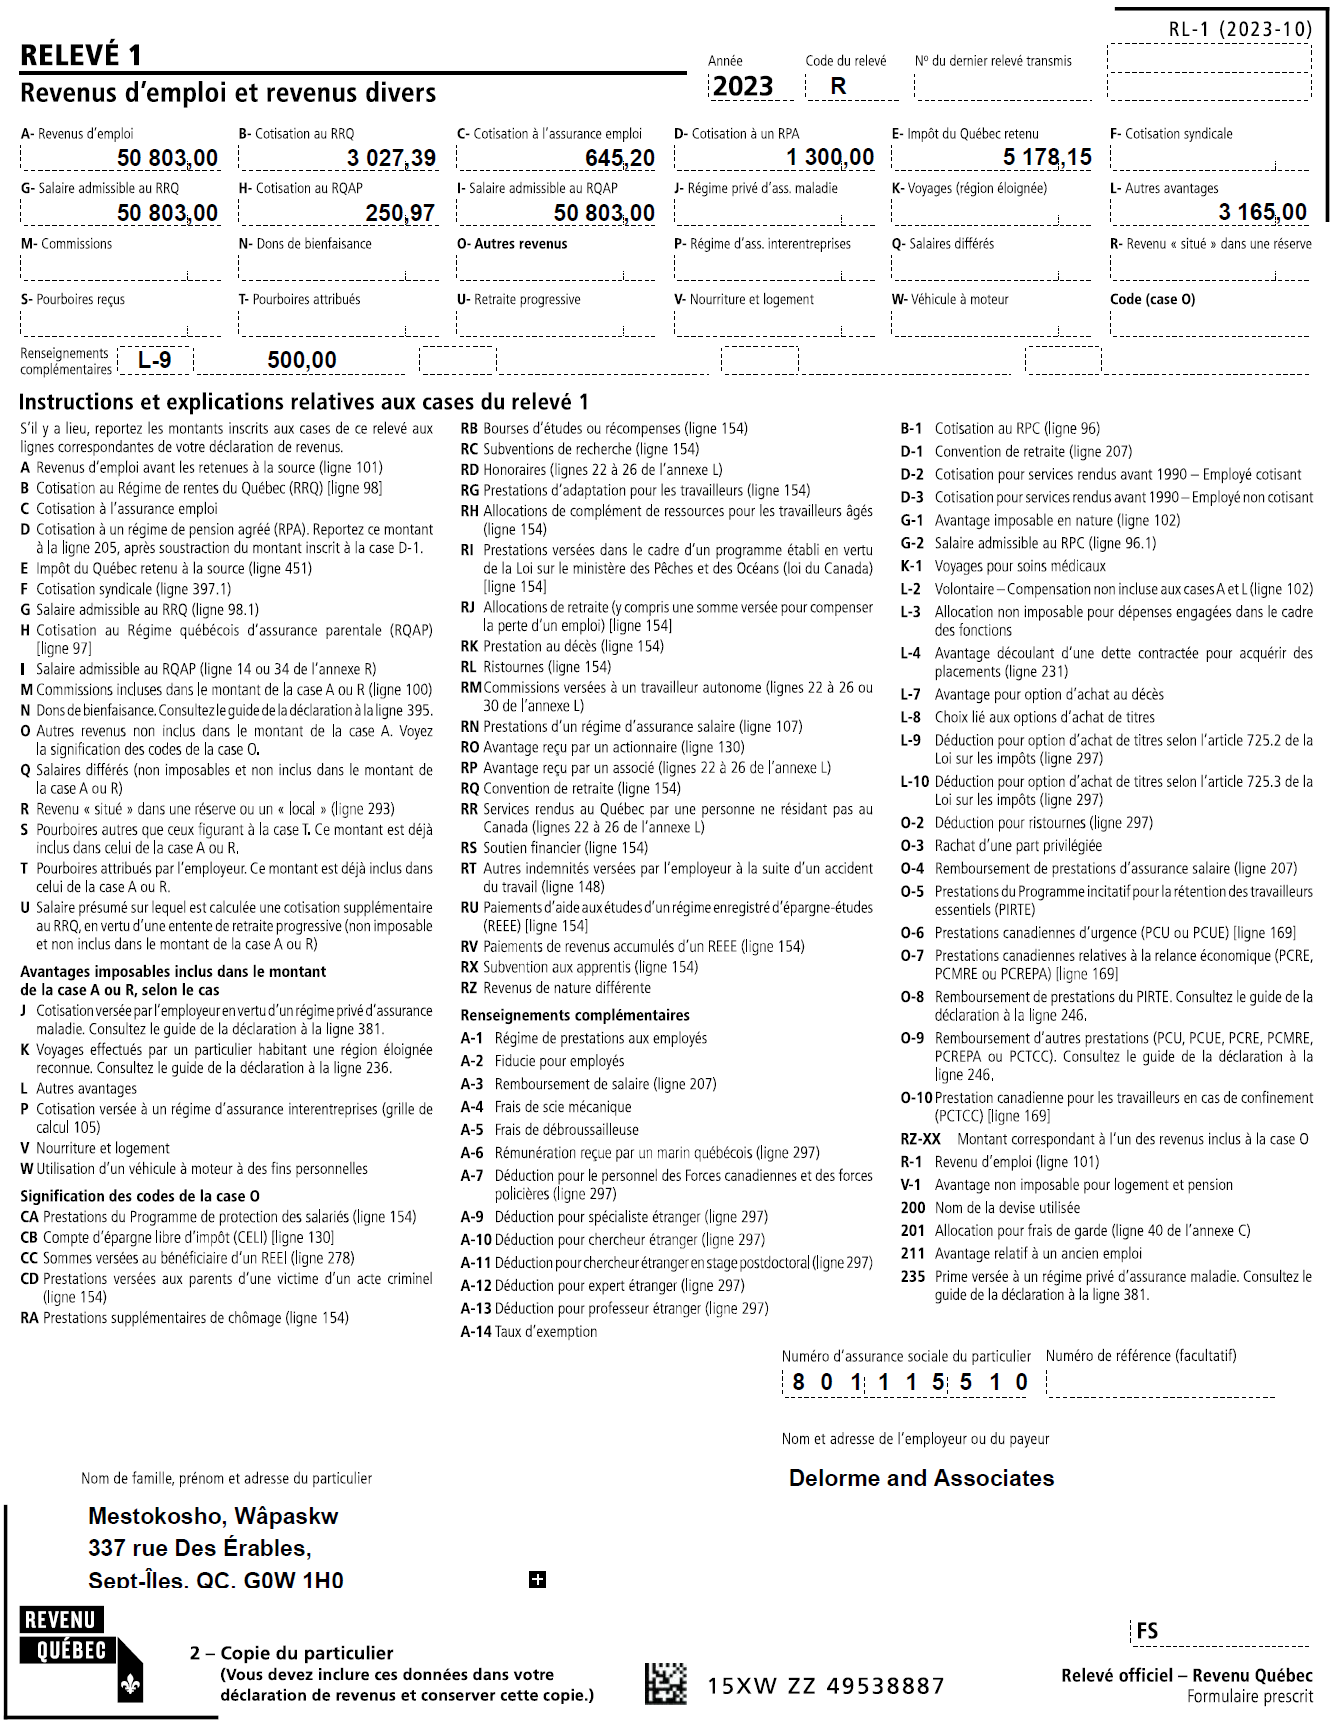
\includegraphics[width=.9\textwidth]{probleme/chapitre-5/Wapaskw-RL1.png}
	\caption[]{Problème, RL-1}
	\label{fig:chap5ProblemeRL1}
\end{figure}
\begin{figure}
	\centering
	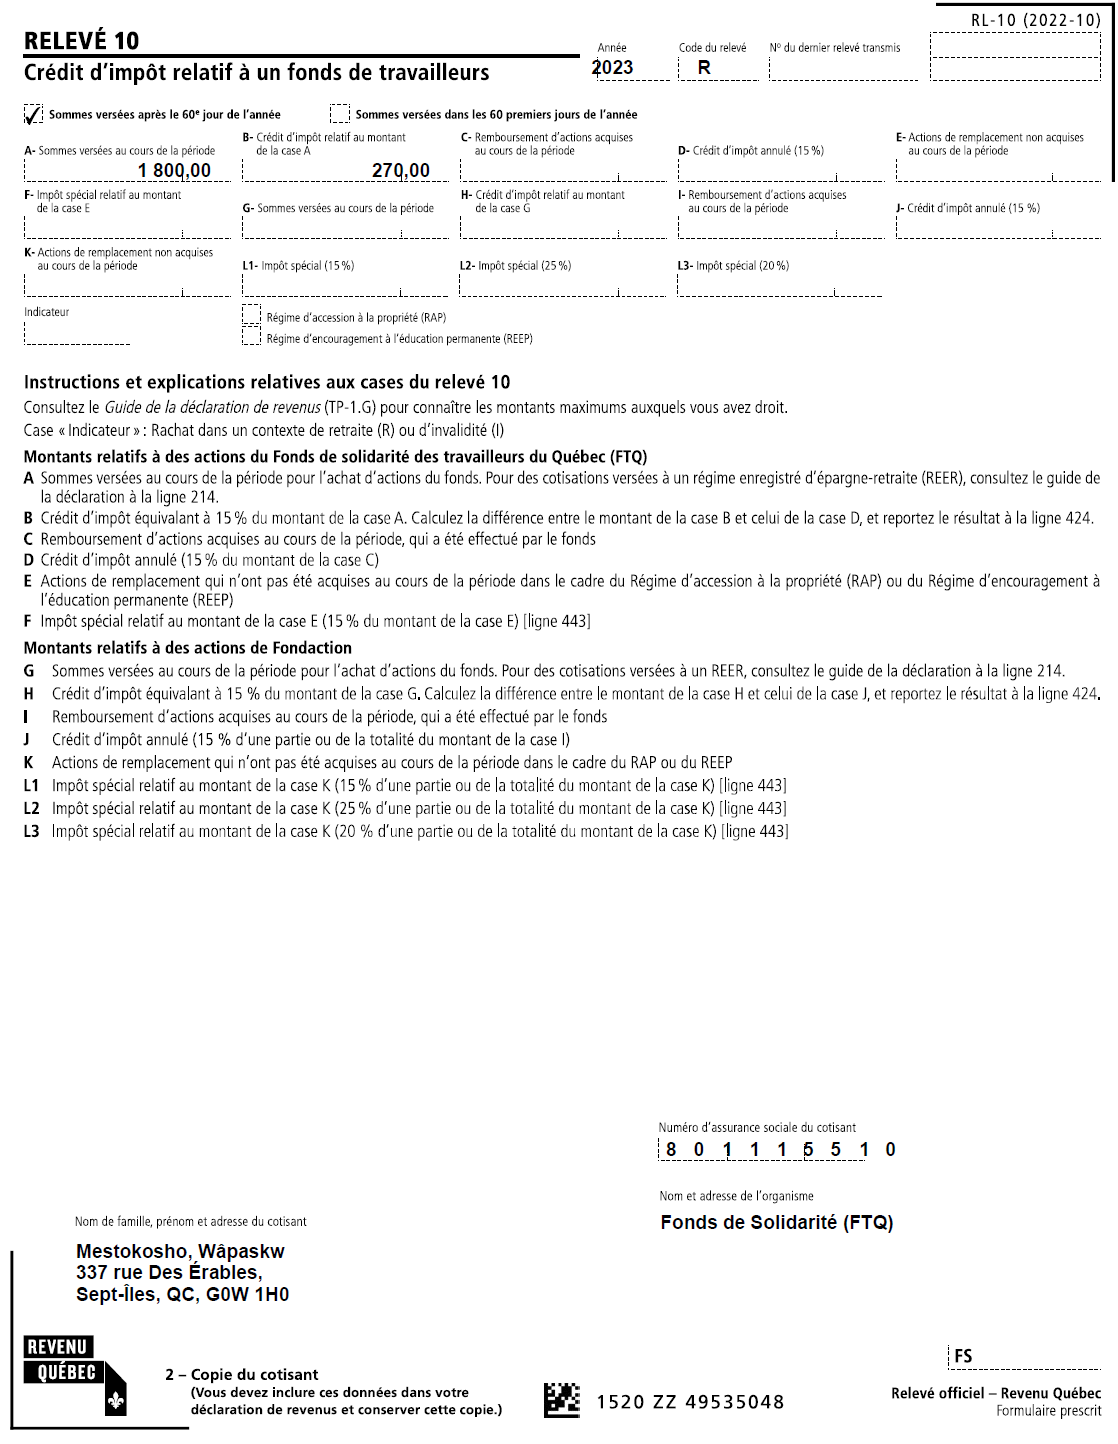
\includegraphics[width=.9\textwidth]{probleme/chapitre-5/Wapaskw-RL10-FTQ.png}
	\caption[]{Problème, RL-10 FTQ}
	\label{fig:chap5ProblemeRL10FTQ}
\end{figure}
\begin{figure}
	\centering
	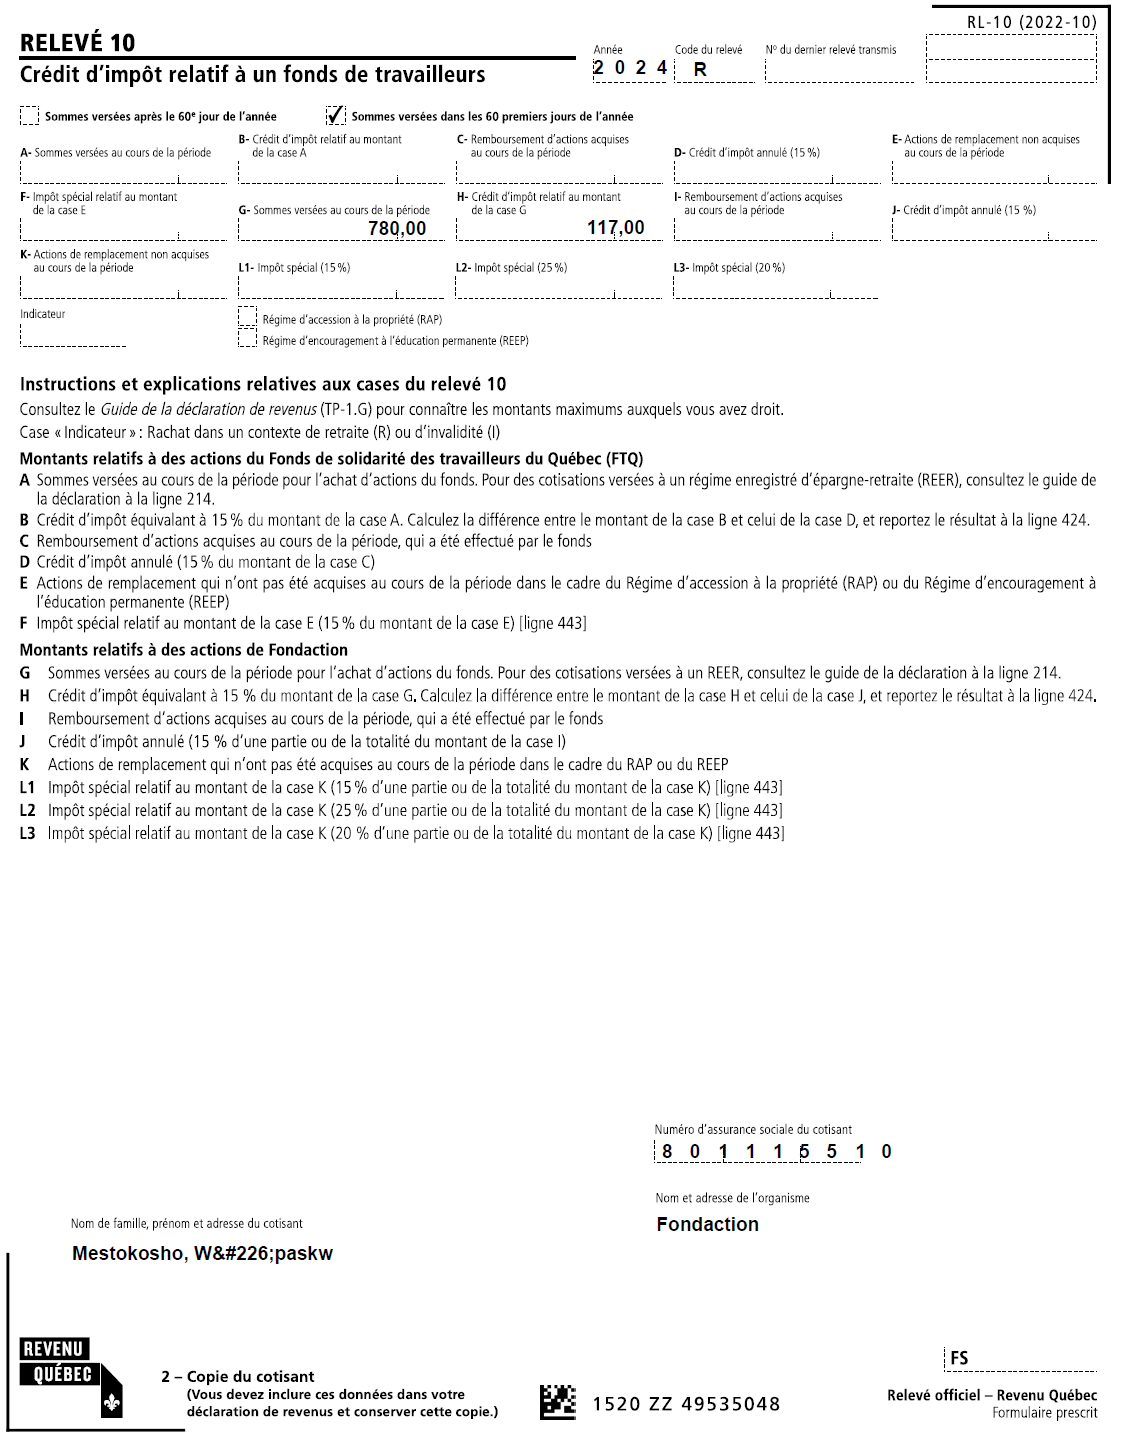
\includegraphics[width=.9\textwidth]{probleme/chapitre-5/Wapaskw-RL10-Fondaction.png}
	\caption[]{Problème, RL-10 Fondaction}
	\label{fig:chap5ProblemeRL10Fondaction}
\end{figure}


\subsection{Feuillets de Wîskacân}
RL-8: Figure \ref{fig:chap5ProblemeRL8}
\begin{figure}
	\centering
	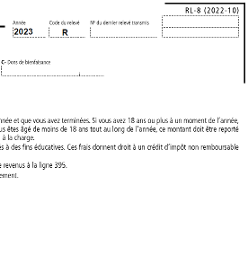
\includegraphics[width=.9\textwidth]{probleme/chapitre-5/Wiskacan-RL8.png}
	\caption[]{Problème, RL-8}
	\label{fig:chap5ProblemeRL8}
\end{figure}


\subsection{Formulaires au fédéral}
Remplissez la grille de calcul de Wâpaskw pour la  \href{https://www.canada.ca/fr/agence-revenu/services/formulaires-publications/trousses-impot-toutes-annees-imposition/trousse-generale-impot-prestations/5000-d1.html}{ligne 41000}, les pages 3 à 8 de sa \href{https://www.canada.ca/fr/agence-revenu/services/formulaires-publications/trousses-impot-toutes-annees-imposition/trousse-generale-impot-prestations/quebec/5005-r.html}{T1} et son \href{https://www.canada.ca/fr/agence-revenu/services/formulaires-publications/trousses-impot-toutes-annees-imposition/trousse-generale-impot-prestations/5000-s5.html}{annexe 5}.

\setcounter{question}{0}
\begin{question}
	Wâpaskw peut-il demander le montant fédéral pour une personne à charge admissible? Expliquez votre réponse.
\end{question}
Wâpaskw peut demander le montant fédéral pour une personne à charge admissible, il est veuf et sa fille Âpikusîs à moins de 18 ans.

\begin{question}
	D'après votre réponse à la question 1, Wâpaskw peut-il demander d'autres montants personnels fédéraux pour ses enfants?
\end{question}
Oui, ligne 30500 pour Âpikusîs, le montant canadien pour aidant naturel pour enfants âgés de moins de 18 ans ayant une déficience, \numprint{2499}~\$.


\subsection{Formulaires du Québec}
Compléter les \href{https://www.revenuquebec.ca/documents/fr/formulaires/tp/2023-12/TP-1.D.GR%282023-12%29.pdf}{grilles de calcul} 201, 401 et 414 de Wâpaskw, ses annexes \href{https://www.revenuquebec.ca/documents/fr/formulaires/tp/2023-12/TP-1.D.A%282023-12%29.pdf}{A}, \href{https://www.revenuquebec.ca/documents/fr/formulaires/tp/2023-12/TP-1.D.B%282023-12%29.pdf}{B}, \href{https://www.revenuquebec.ca/documents/fr/formulaires/tp/2023-12/TP-1.D.D%282023-12%29.pdf}{D} et \href{https://www.revenuquebec.ca/documents/fr/formulaires/tp/2023-12/TP-1.D.K%282023-12%29.pdf}{K}, ainsi que les pages 2 à 4 de la \href{https://www.revenuquebec.ca/documents/fr/formulaires/tp/2023-12/TP-1.D%282023-12%29.pdf}{TP-1}


\subsection{Questions}
\begin{question}
	Wâpaskw a-t-il droit au montant québécois pour une personne vivant seule? Expliquez votre réponse.
\end{question}
Wâpaskw a droit au montant québécois pour une personne vivant seule car Âpikusîs est mineure, Wîskacân est majeur mais il poursuit à temps plein des études postsecondaires, et il a un logement domestique autonome, il a un relevé~31.

\begin{question}
	Wâpaskw est-il admissible au montant supplémentaire pour personne vivant seule au Québec? Expliquez votre réponse.
\end{question}
Wâpaskw n'est admissible au montant supplémentaire pour personne vivant seule ligne 361 car au mois de décembre il a reçu l'Allocation famille versée par Retraite Québec, il a un enfant à charge de moins de 18 ans qui réside avec lui.

\begin{question}
	Si Wâpaskw peut demander soit le montant pour une personne vivant seule, soit le montant supplémentaire pour une personne vivant seule, quel montant peut-il demander? Utilisez l'annexe B ci-dessous pour répondre à cette question.
\end{question}
Wâpaskw peut demander le montant pour une personne vivant seule, \numprint{1969}~\$, il a seulement des enfants mineurs ou des enfants majeurs aux études postsecondaires à plein temps. Il ne peut pas demander le montant supplémentaire pour une personne vivant seule car il vit avec un enfant mineur.

\begin{question}
	Comment Wâpaskw peut-il réclamer le montant que Wîskacân lui a transféré?
\end{question}
Wâpaskw peut réclamer le montant que Wîskacân lui a transféré (annexe S) en remplissant la partie B de l'annexe A, et reportant le montant à ligne 367 de sa déclaration. 

\begin{question}
	Si Wîskacân fait une demande rétroactive du CIS en date de septembre 2023, recevra-t-il tous les paiements des années passées auxquels il était admissible?
\end{question}
Wîskacân peut faire une demande seulement pour les quatre dernières années, de 2020 à 2023. Il a eu 18 ans en 2020, sa première demande peut être faite dans sa déclaration de 2020.
